%
% File emnlp2020.tex
%
%% Based on the style files for ACL 2020, which were
%% Based on the style files for ACL 2018, NAACL 2018/19, which were
%% Based on the style files for ACL-2015, with some improvements
%%  taken from the NAACL-2016 style
%% Based on the style files for ACL-2014, which were, in turn,
%% based on ACL-2013, ACL-2012, ACL-2011, ACL-2010, ACL-IJCNLP-2009,
%% EACL-2009, IJCNLP-2008...
%% Based on the style files for EACL 2006 by 
%%e.agirre@ehu.es or Sergi.Balari@uab.es
%% and that of ACL 08 by Joakim Nivre and Noah Smith

\documentclass[11pt,a4paper]{article}
\usepackage[hyperref]{emnlp2020}
\usepackage{times}
\usepackage{latexsym}
\usepackage{graphicx}
\usepackage{hyperref}
\usepackage{placeins}

\let\Oldsection\section
\renewcommand{\section}{\FloatBarrier\Oldsection}

\let\Oldsubsection\subsection
\renewcommand{\subsection}{\FloatBarrier\Oldsubsection}

\let\Oldsubsubsection\subsubsection
\renewcommand{\subsubsection}{\FloatBarrier\Oldsubsubsection}
\renewcommand{\UrlFont}{\ttfamily\small}

% This is not strictly necessary, and may be commented out,
% but it will improve the layout of the manuscript,
% and will typically save some space.
\usepackage{microtype}

%\aclfinalcopy % Uncomment this line for the final submission
%\def\aclpaperid{***} %  Enter the acl Paper ID here

%\setlength\titlebox{5cm}
% You can expand the titlebox if you need extra space
% to show all the authors. Please do not make the titlebox
% smaller than 5cm (the original size); we will check this
% in the camera-ready version and ask you to change it back.

\newcommand\BibTeX{B\textsc{ib}\TeX}

\title{Prediction of Community Approval of Reddit Posts}

\author{Runxuan Jiang \thanks{\, University of Michigan Department of EECS} \\
  \texttt{runxuanj@umich.edu} \\
  \And
  Tianyi Li \footnotemark[1]\\
  \texttt{litianyi@umich.edu} \\
  \And 
  Tianchen Ye \footnotemark[1]\\
  \texttt{jackye@umich.edu}}

\date{}

\begin{document}
\maketitle
\begin{abstract}
    In this study, we predict of the approval of a new post in a specific community within the social media platform Reddit. We divide this task into three sub-tasks: predicting whether the net amount of upvotes on the post will surpass a certain threshold, predicting directly the upvote ratio the post will receive, and predicting which of three ranges the upvote ratio will fall into. We attempt to build models for these tasks using only textual data from the Reddit posts themselves, including the title and text, avoiding any features that may only be collected after the post has been released such as comment count. We also introduce a custom loss function for dealing with the imbalanced nature of Reddit upvote data. We train and test our models on several university subreddits and find that our models perform reasonably well with respect to a random baseline.
\end{abstract}

\Oldsection{Introduction}
    The task of deterimining the attitudes and approval of a certain community towards an idea is often very useful, and can lead to insights in economics, finance, and public policy. At the same time, this task can be very difficult since it involves gathering the opinions of a large amount of people within one community, and obtaining an accurate representation of someone's "attitude" is a non-trivial task. The first issue can be resolved with the rise of social media, specifically Reddit, where forums are already organized into communities surrounding a single topic. In particular, university subreddits have grown exponentially in the past few years, with subreddits like r/berkeley reaching over 100,000 members. While it is still difficult to determine users' attitudes using this data, the problem can be simplified to instead analyze the approval of users in a subreddit towards a specific post. The goal of this project is thus to create and analyze models that, given a textual post, predicts the approval of the post within a certain subreddit. 

    Previous works have conducted similar exploration on Reddit data, almost all of which attempt to predict the net upvote count (the number of upvotes minus downvotes) of a post using regression or binary classification \citep{Segall2012,Shuaibi2019,Terentiev2014}. However, many of these studies collect their data as a set of posts from a "pool" of different subreddits, and create models across all these subreddits. Often times such models perform poorly, especially on regression of the net upvote count, where the RMSE across such models is almost always higher than 100 \citep{Segall2012,Shuaibi2019}. Additionally, some works use features that can only be known after the post has been created, such as the number of comments \citep{Shuaibi2019}.

    To address the task of predicting the approval of a post within a certain subreddit, we first define two metrics that we believe are correlated with a posts' approval: net upvote count (upvotes - downvotes) and upvote ratio (upvotes / total votes). We focus more heavily on upvote ratio since it is more related to the notion of a post's "approval". We specifically study three sub-tasks involving these metrics:
    \begin{enumerate}
        \item We pose the prediction of net upvote count as a binary classification task, where we predict whether the net upvote count of a post will exceed a certain threshold.
        \item We pose the prediction of upvote ratio as a regression task, where we predict directly the upvote ratio of a post.
        \item We also consider the prediction of upvote ratio as a classification task, where we predict which of three ranges the upvote ratio of a post will fall into.
    \end{enumerate}
    In the rest of this paper, we may sometimes refer to each of these three sub-tasks as "task 1", "task 2", and "task 3", respectively.
    
    For the regression task, we further introduce a custom loss function and smoothing techniques for handling imbalanced data. We then train subreddit-specific models for each task using text data collected from university related subreddits including r/uofm, r/berkeley, r/uwaterloo, and r/UTAustin. We specifically chose university subreddits since we felt that the type of posts in these subreddits will be more homogenous over time, as compared to subreddits like r/news or r/politics which will vary greatly by current events. The models used include feed-forward neural networks for regression, and k-nearest neighbors (KNN), gaussian mixture models (GMM), random forest classifier (RFC), and neural networks for classification. In terms of feature generation, our models are trained solely using the textual information (title and text) of each post.

    We then evaluate our model performance on posts not seen before during training, and interpret the models to identify trends within each subreddit. For the  first task (binary classification of net upvote count), our neural network model achieved an accuracy of over 0.7 for each subreddit. For regression of upvote ratio, our neural network model consistently had a mean absolute error (MAE) of around 0.2. And for three-class classification of upvote ratio our GMM model was able to achieve an accuracy of 0.5 for most subreddits. Note that our models are trained solely on textual post data and does not use any features that depend on future interaction with the post (such as number of comments). Furthermore, after a thorough search we have not found any other works that focus on the prediction of upvote ratio, so our models for regression and classification of upvote ratio may act as a baseline for future work in this area.

    The paper is organized as follows. We will first discuss in more detail related works. We will then discuss how we collected and cleaned our data in the \hyperref[sec:data]{"data"} section and presetn visualizations of our data. Next in \hyperref[sec:methods]{"methods"} we discuss how we chose our metrics and features. In \hyperref[sec:algorithms]{"algorithms"}, we will discuss each of the learning algorithms we used for each of the three tasks. We then discuss the performance of the models and how we interpreted the models in \hyperref[sec:results]{"results and discussion"}. Finally, we discuss some ethical issues related to this project in \hyperref[sec:ethics]{"ethical considerations"}.



\Oldsection{Related work}
    There have been several previous works involving supervised learning tasks on Reddit data, specifically with predicting Reddit post popularity (number of upvotes - downvotes of a post).

    \citet{Segall2012} studied the prediction of net upvote count both as a multi-class classification problem (where the classes are different ranges of net upvote count) and a regression problem. The study used a random sample of over 2 million reddit posts, and used features including title and text embedded using TF-IDF, author, time created, and whether the post is marked as "over 18". The study tried several techniques, including naive bayes and multi-class SVM for classification, and linear regression for regression.
    
    \citet{Shuaibi2019} also studied the prediction of net upvote count, focusing mainly on regression techniques. The study only utilized the title of the each post as the only textual feature, and utilized other features like number of comments and whether the post was given any Reddit rewards. The study also used engineered features such as the length of the title and the sentiment of the title. Three regression models were trained on posts across several subreddits from the first 6 months of 2018, including linear regression, KNN regression, and random forest regression.



\Oldsection{Data}
\label{sec:data}

    \Oldsubsection{Data collection}
    We collected all posts prior to March 2022 in the subreddits r/uofm, r/berkeley, r/uwaterloo, and r/UTAustin using Reddit's API, using the pushshift.io library \citep{Pushshiftio2020}. For each post, we collected the title, text , upvote scores, upvote ratio, text\_only, and number of comments of each post. Note that text\_only is a boolean that is set to true if a post does not have any non-textual content (like images). The distribution of net upvote count for r/uofm is shown in figure \ref{fig:uofm_upvotes}. Histograms for other subreddits can be found in \ref{sec:appdata}. Using the upvote ratio and net upvote count, we were also able to calculate the total number of votes in general (upvotes + downvotes) for each post.

    \begin{figure*}
        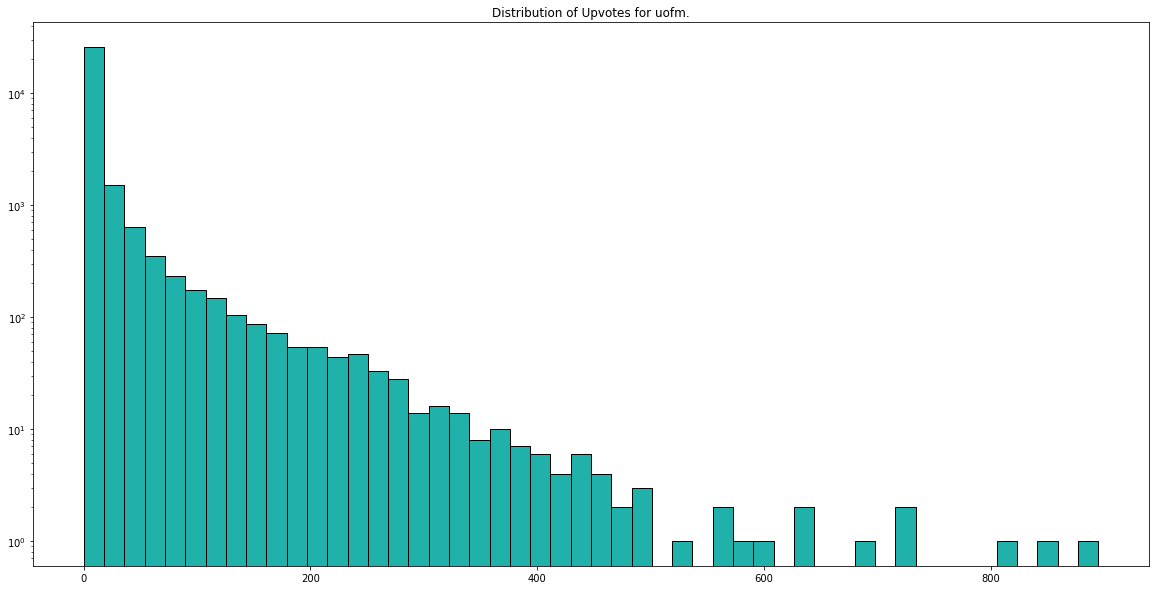
\includegraphics[width=\textwidth]{uofm_upvotes.png}
        \caption{Distribution of net upvote count for r/uofm.}
        \label{fig:uofm_upvotes}
    \end{figure*}

    \Oldsubsection{Data cleaning and filtering}
    Next, we filtered the data by only keeping posts where text\_only is set to true, since we plan on working only with posts that use textual data. We also filtered out posts with less than 5 comments and less than 16 total votes (upvotes + downvotes). This is because by default posts will have exactly one upvote (from the user who posted it) and would thus have an upvote ratio of 1. However, this does not reflect the community as a whole and thus we only want to maintain posts with a certain number of community interactions.

    We then cleaned our data by concatenating the title and text of each post, since some posts only have a title. We also converted any posts where the text or title were '[deleted]' or '[removed]' to an empty string, and converted all text to lowercase. A histogram of upvote ratios for r/uofm is shown in figure \ref{fig:uofm_ratio1}.

    We then split our data into a training set and test set for each subreddit by first shuffling the data and then choosing the first 80\% of the data to be the training set and the remaining 20\% to be the test set. When training models for each of our experiments, we exclusively used the training set, and we evaluted each model using the test set.

    \begin{figure*}
        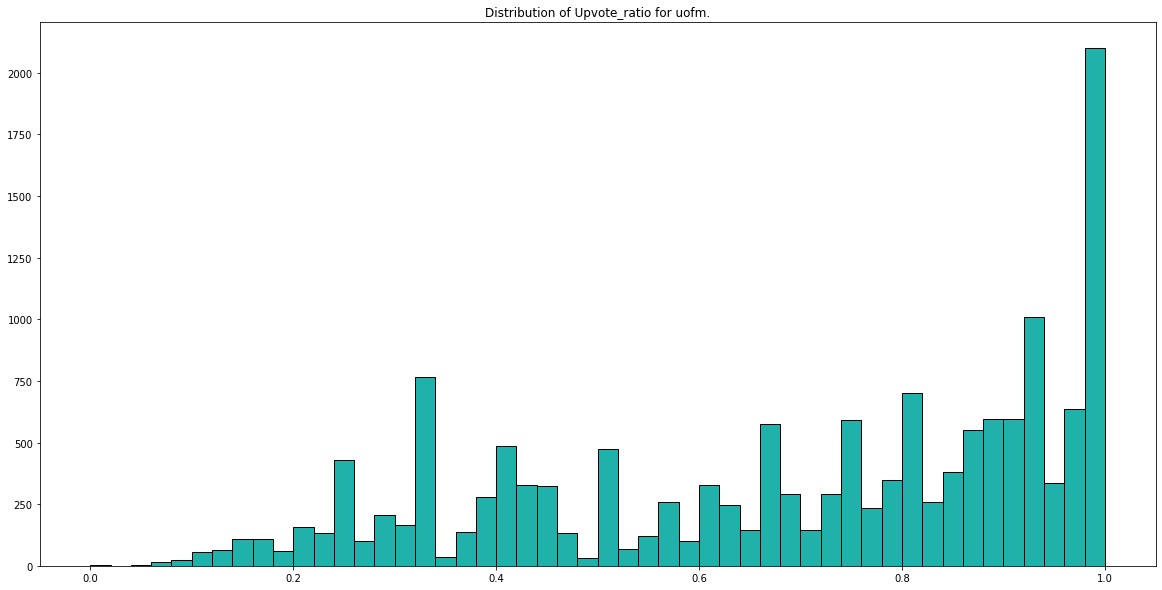
\includegraphics[width=\textwidth]{uofm_ratio1.png}
        \caption{Distribution of upvote ratio after data cleaning for r/uofm.}
        \label{fig:uofm_ratio1}
    \end{figure*}


\Oldsection{Methods}
\label{sec:methods}
    \Oldsubsection{Metrics Used}
        We decide to use both net upvote count and upvote ratio as our metric for a post's approval. We chose to use net upvote count because it is the same metric used by Reddit's algorithm for determining which posts are "popular" and will be more likely to show up on the front page of the subreddit. However, this metric does not directly align with a post's approval since a post with a high net upvote count could have no downvotes, or it could have a significant amount of downvotes. Furthermore, the previous work by \citet{Shuaibi2019} has shown that predicting net upvote count is difficult, which is likely caused by the fact that the distribution of net upvote count is highly skewed, as seen in figure \ref{fig:uofm_upvotes}. Thus, we only chose to predict net upvote count as a binary classification task and focus more on upvote ratio. Upvote ratio directly measures the percentage of users who approved of the post, conditioned on the fact that the user interacted (or voted) on the post. Since we are not able to access data on how many people viewed the post (but did not interact with the post), we believe this is the closest metric we could obtain for gauging the approval of the subreddit towards the post.

        

    \Oldsubsection{Feature Generation}
        In order to be used as input to our models, we converted our textual posts into fixed length numerical vectors using a pretrained attention model called sentence Bert (or SBert) \citep{Sbert2019}, which achieves state-of-the-art performance on sentence-pair regression tasks like semantic textual similarity. The embedding method applied bi-directional attention layers, which guides the embedding layer to try to “focus” on words that contain more information, and then filter out the information through unsupervised learning. In this particular case, we applied the pre-trained model all-MiniLM-L6-v2, which converts each post into a 384-dimensional vector. Each vector is of unit length and the model is designed to assign vectors of similar cosine similarity to similar input text.


\Oldsection{Algorithms}
\label{sec:algorithms}
    We now describe in detail each sub-task as well as the algorithms used.

    \Oldsubsection{Task 1: Binary Classification of Net Upvote Count}
    In this experiment, we consider our problem as a classification task to tell whether a certain post will be popular or not based on the number of net upvotes. We define posts that are being popular and under hot discussions as those with net upvotes larger or equal to 5, and those being tedious with net upvotes less or equal to 1. The threshold of tediousness being one is because each post will automatically receive one upvote from the user itself, so posts with one upvote basically indicates there is no other user looking into the post. Because of the skew of the dataset, there are many more posts with the number of upvotes in the tedious category, and thus we selected the same amount of data points from the two categories to deal with the imbalance. 
    Next, we applied a deep neural network to solve the classification problem. Visually, the model follows the pipeline shown in figure \ref{fig:nnet}.

    \begin{figure*}
        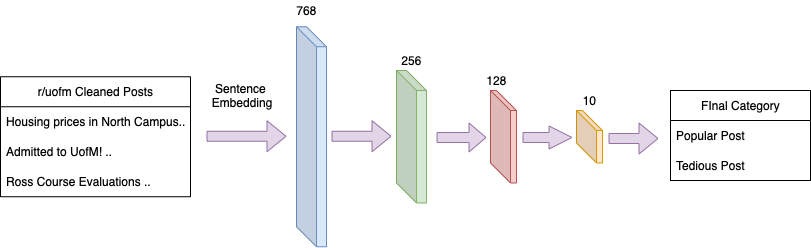
\includegraphics[width=\textwidth]{nnet.png}
        \caption{Feed-forward neural network architecture used in task 1.}
        \label{fig:nnet}
    \end{figure*}
    
    Between each layer, we use a ReLU activation function to add non-linearity, and a dropout layer to enhance the generality of the model. At the end of the model, we applied sigmoid for the classification task. The model is trained using a binary cross-entropy loss function.

    \Oldsubsection{Task 2: Regression of Upvote Ratio}
    In this task, we try to predict the upvote ratio for a post by directly predicting the upvote ratio value. We train a neural network identical to the one in task 1 shown in figure \ref{fig:nnet}, except for the last layer maps to a single scalar value representing the upvote ratio, rather than a 2-dimensional vector. At first, we train our neural network using the mean absolute error (MAE) as our loss function:

    \[MAE = \frac{1}{n} \sum_{i=1}^n |\hat{y_i} - y_i|.\]

    where $n$ is the size of one batch, $\hat{y_i}$ is the predicted upvote ratio for datapoint $i$, and $y_i$ is the true upvote ratio for datapoint $i$. For this task only, we further filter our data to only include posts with a total number of votes greater than 20, to further reduce the skewness of the distribution of upvote ratio.

    \begin{figure*}
        \begin{minipage}{0.5\textwidth}
            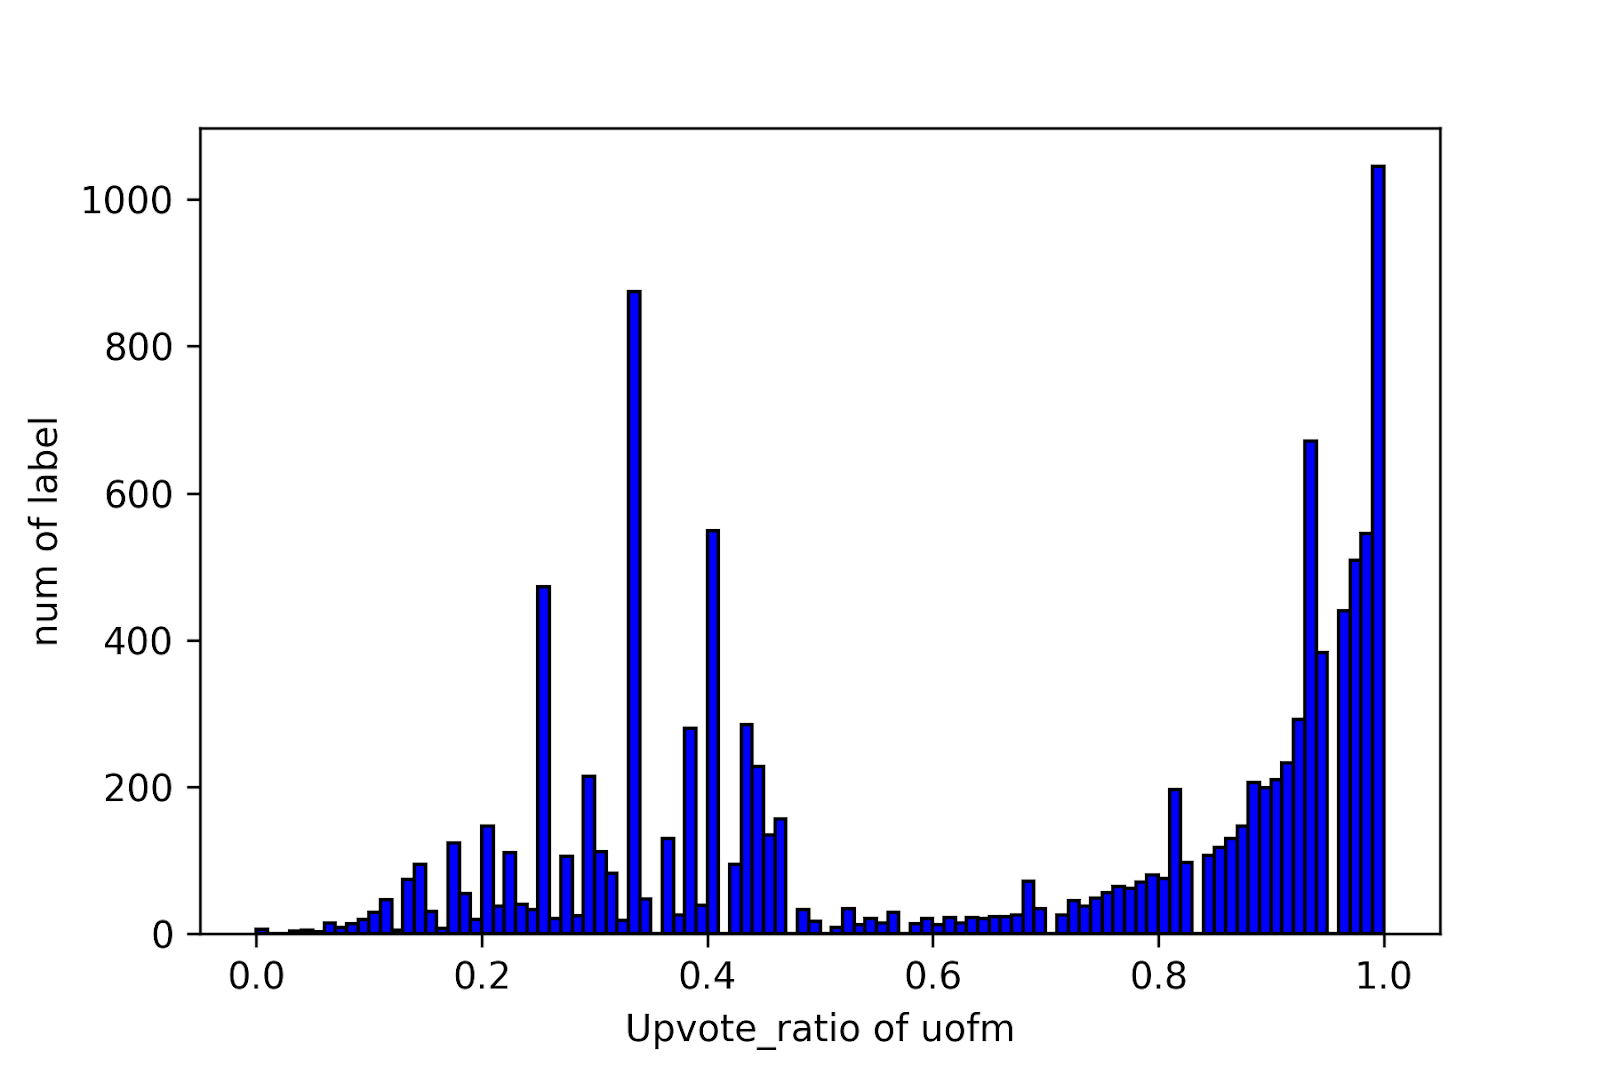
\includegraphics[width=\textwidth]{uofm_task2true_nonsmooth.png}
        \end{minipage}
        \begin{minipage}{0.5\textwidth}
            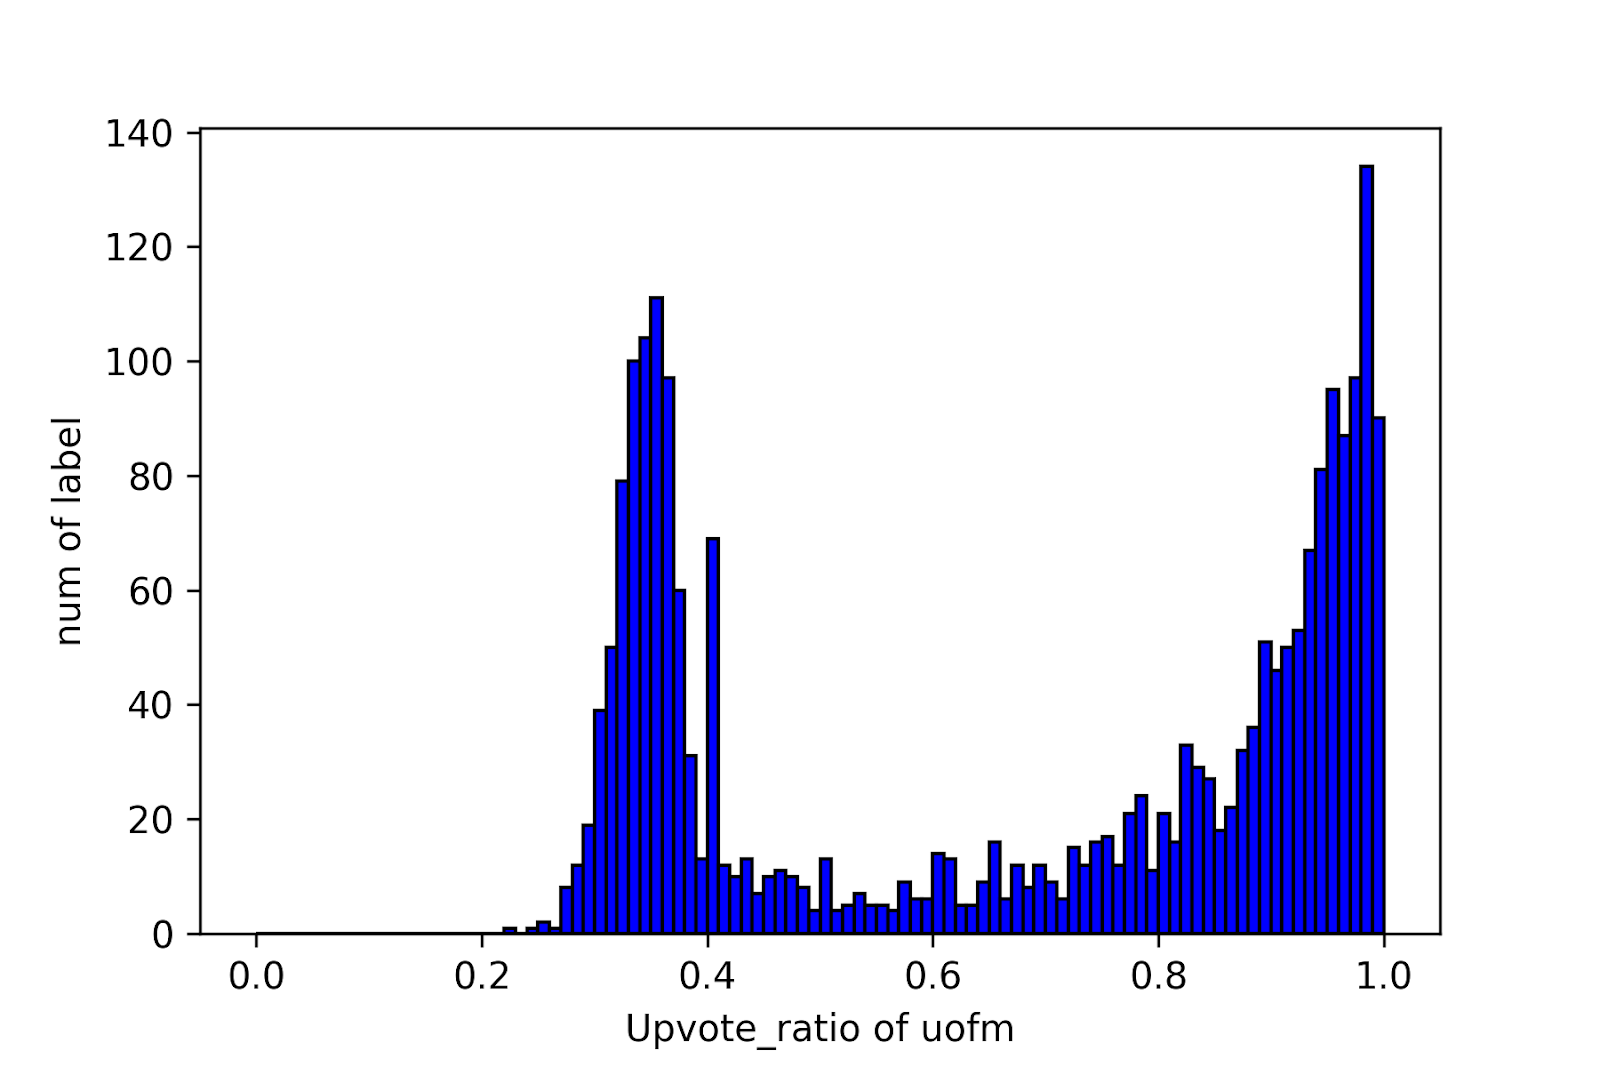
\includegraphics[width=\textwidth]{uofm_task2pred_nonsmooth.png}
        \end{minipage}

        \caption{True (left) and predicted (right) distributions of upvote ratios for r/uofm using model trained on MAE loss.}

        \label{fig:task2_before}
    \end{figure*}

    However, by comparing the histograms of the actual upvote ratio and the predicted upvote ratio, we find that most of the predicted values are in the interval [0.3, 0.4] and [0.9,1.0], as seen in figure \ref{fig:task2_before}. This is mainly due to the imbalanced training dataset. In order to minimize the loss function (i.e. Mean Absolute Error), our model tends to predict a value that has the highest occurring probability. However, the model trained is highly biased and failed to recognize the actual pattern of the data, as there are almost no predictions below 0.2. A model like this is not desired because it failed to predict values with low occurring probability.

    To solve this problem, we decided to design a new loss function that can lower the influence of data with high occurrence. We refer to the new loss function as the Weighted Mean Absolute Error (WMAE), and it is calculated as follows:

    \[WMAE = \frac{1}{n} \sum_{i=1}^n \frac{|\hat{y_i} - y_i|}{W(y_i)}.\]
    where 
    \[W(y_i) = \frac{\log P(y_i)}{\sum_{j=1}^n \log P(y_j)}.\]

    where $P(y_i)$ is the probability of $y_i$ occuring among the true labels. Since the true labels occur within a continuous range, we fit a continuous probability distribution over the distribution of our true labels. We first smooth the data by adding or subtracting 0.03 at random to the true upvote ratios. Then, we utilize the Kernel Density function provided by scikit-learn \citep{scikit-learn2011} to fit a density distribution over the upvote ratios. The fitted density distribution for r/uofm can be seen in figure \ref{fig:density}. We then use the value of the density function at $y_i$ for $P(y_i)$. 

    \begin{figure}
        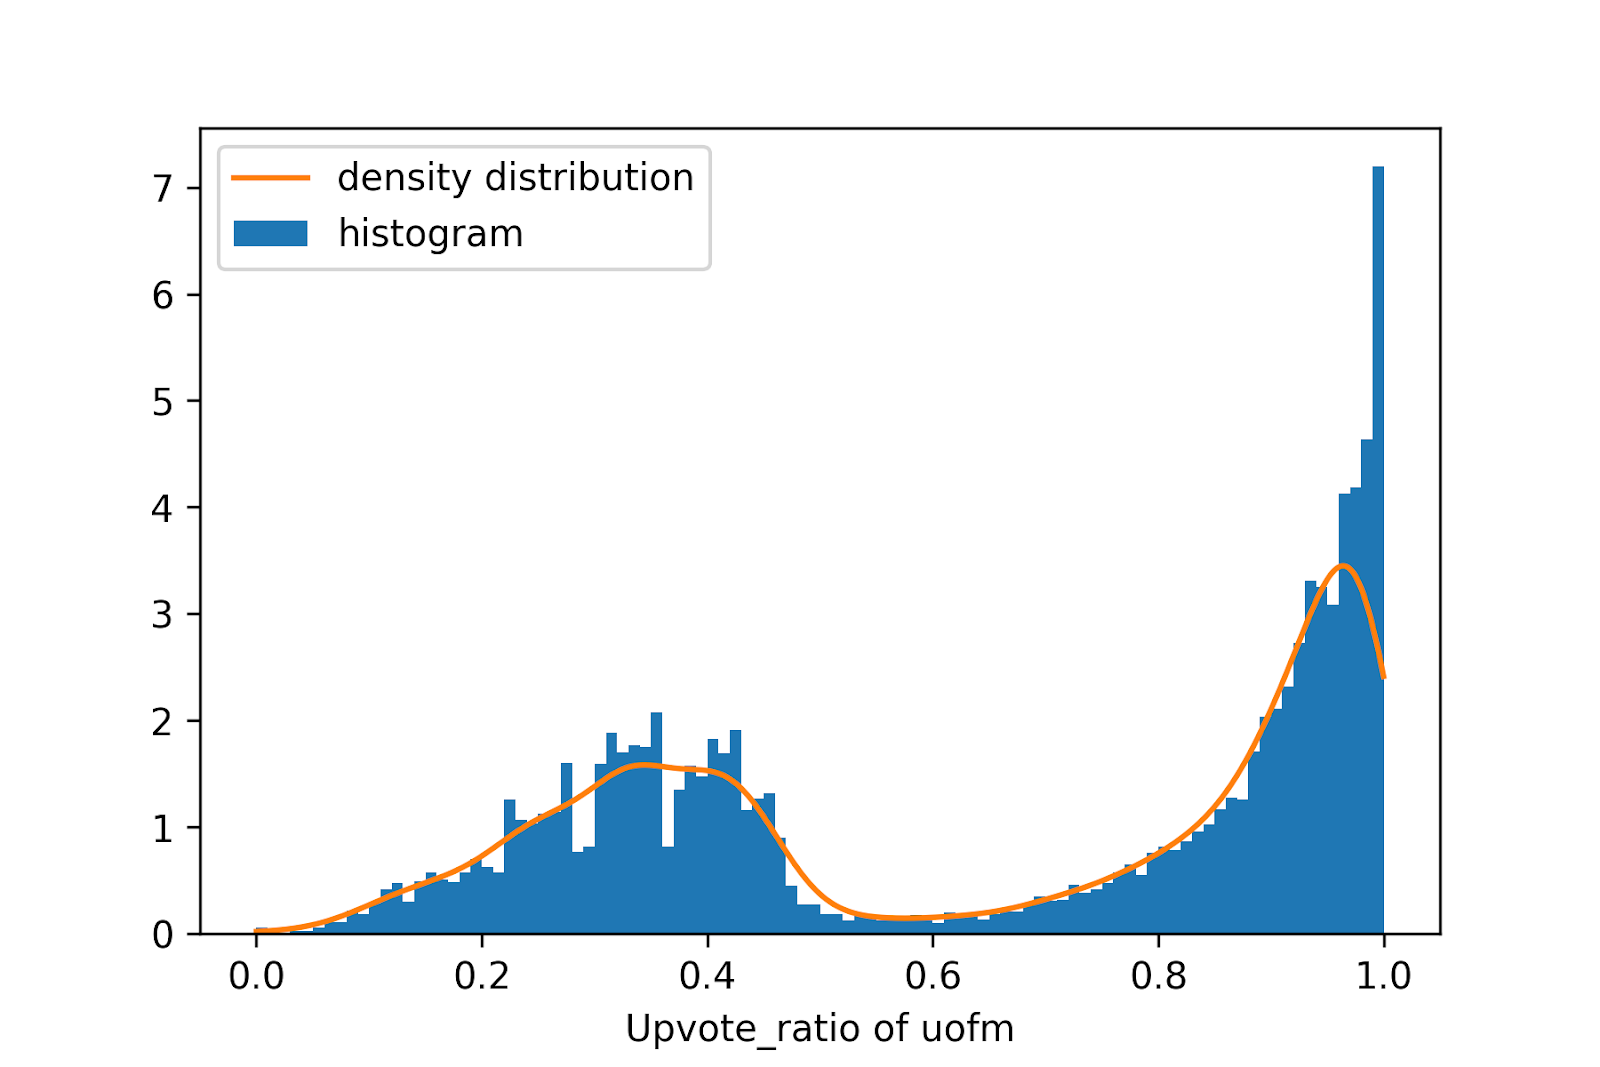
\includegraphics[width=0.5\textwidth]{uofm_task2true_smooth.png}
        \caption{Smoothed distribution of upvote ratio (labels) and fitted kernel density for r/uofm.}
        \label{fig:density}
    \end{figure}

    We then trained the neural network using this loss function. We see that the result distribution of predicted upvote ratios has higher occurances in ranges with low label occurances, as seen in figure \ref{fig:task2_after}.
    

    \begin{figure}
        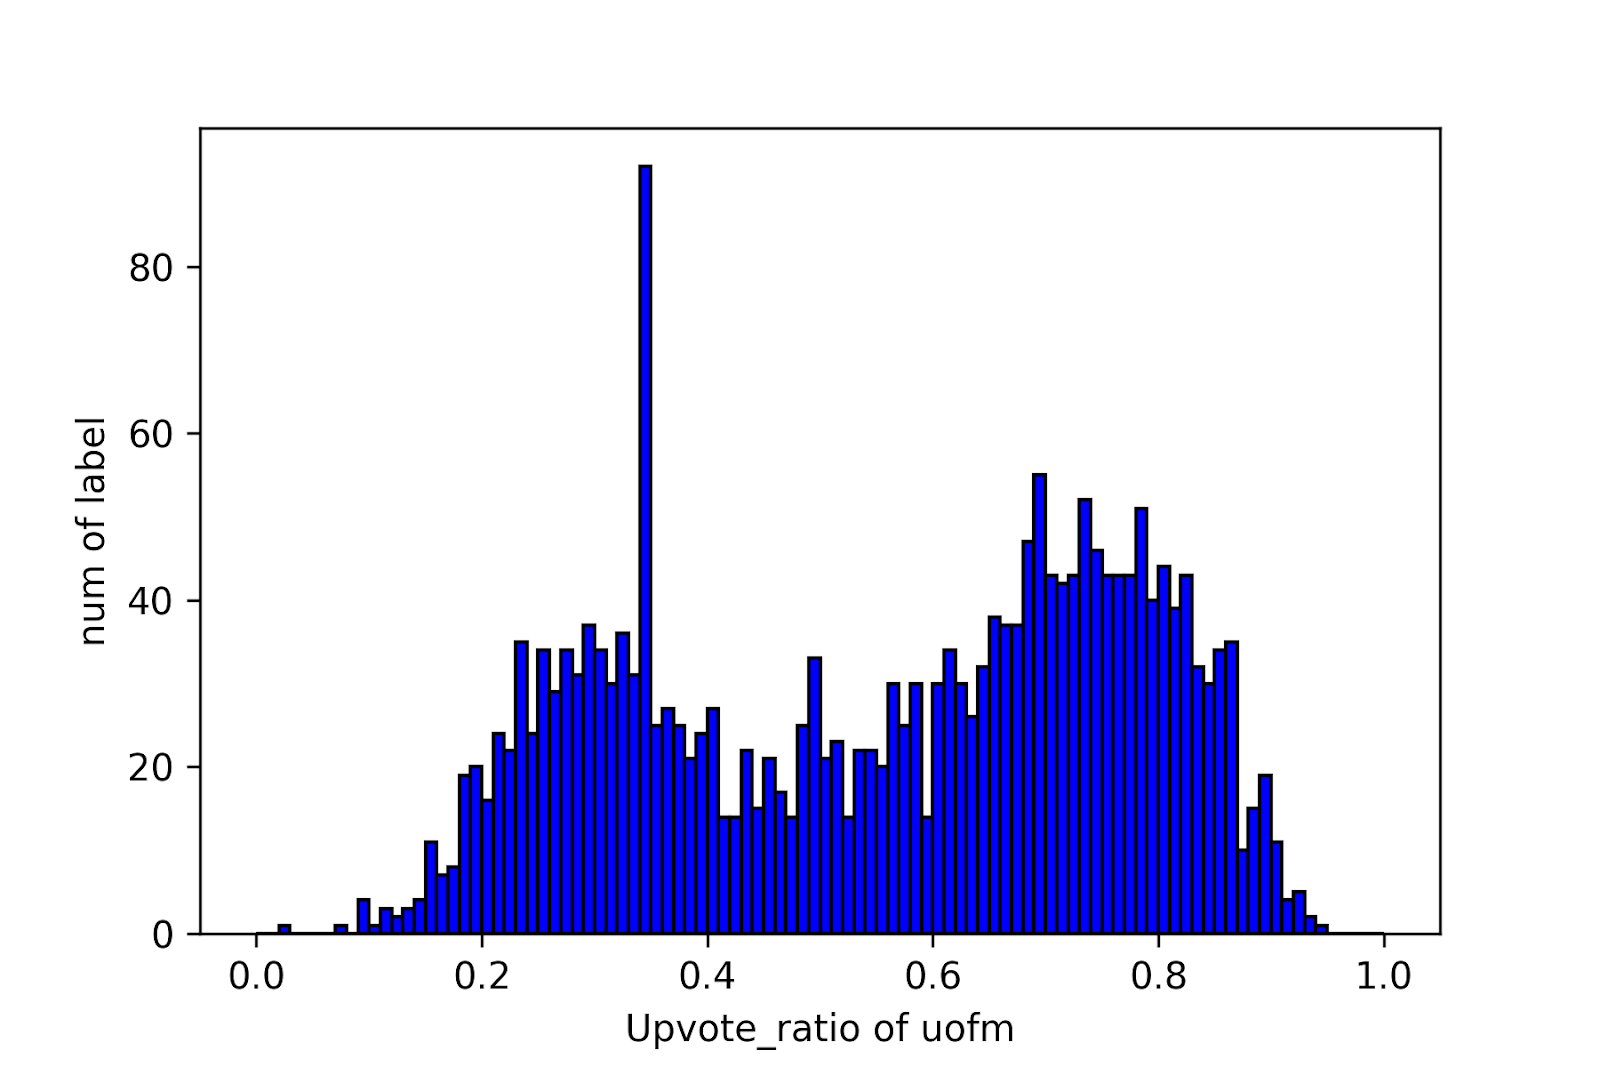
\includegraphics[width=0.5\textwidth]{uofm_task2pred_smooth.png}
        \caption{Distribution of predicted upvote ratio after training using weighted MAE.}
        \label{fig:task2_after}
    \end{figure}

    For figures of the distribution of predicted upvote ratio for each of the four subreddits, see \ref{sec:appdistr}.

    \Oldsubsection{Task 3: Classification of Upvote Ratio}
        In this experiment, we pose the predict of upvote ratio as a classification problem where the goal is to predict which of three ranges of values the upvote ratio for a post falls into. The ranges chosen for this task are (0, 0.5), (0.5, 0.8), and (0.8, 1). The first range corresponds to posts that have more downvotes than upvotes and thus can be categorized as "negative approval". The second category has slightly more upvotes than downvotes and can be categorized as "mild approval" and the third category can be categorized as "high approval". We specifically chose these ranges so that each range can be reasonably correlated with a level of approval, while keeping the data somewhat balanced between the classes. Note that due to the skewness of the data, the highest range still remains with the largest proportion compared to the other ranges. The distribution of the test data for each subreddit among these classes are detailed in figure \ref{fig:ranges}

        \begin{figure}
            \begin{tabular}{ |c|c|c|c| }
                \hline
                subreddit / range& (0, 0.5) & (0.5, 0.8) & (0.8, 1) \\
                \hline
                r/uofm & 3694 & 3220 & 5514 \\
                \hline
                r/berkeley & 6591 & 6724 & 11963 \\
                \hline
                r/uwaterloo & 15247 & 19470 & 22255 \\
                \hline
                r/UTAustin & 3229 & 3410 & 7189 \\
                \hline
            \end{tabular}
            \caption{Distribution of upvote ratio of posts across three different classification ranges for each subreddit.}
            \label{fig:ranges}
        \end{figure}

        For each subreddit, we train four different classifiers on the training set and evaluate on the test set. The classifiers include (hyperparameters selected after tuning):

        \begin{itemize}
            \item K nearest neighbors classifier - the predicted label for each input is the most commonly seen label of the 20 datapoints closest to the input (by Euclidean distance) in the training set.
            \item Random forest classifier - ensemble of 128 decision trees.
            \item Feed forward neural network trained using softmax function and Adam optimizer with the following layers:
            \begin{itemize}
                \item linear(384, 128) $\rightarrow$ ReLU $\rightarrow$ dropout
                \item linear(128, 64) $\rightarrow$ ReLU $\rightarrow$dropout
                \item linear(64, 3) $\rightarrow$ ReLU
            \end{itemize}
            \item Guassian mixture model where each class is modeled by a GMM with 2 components.
        \end{itemize}
        

\Oldsection{Results and Discussion}
\label{sec:results}
    In this section, we discuss the performance of our models in each sub-task.

    \Oldsubsection{Task 1: Binary Classification of Net Upvote Count}
    The results for the neural network model on each of the four subreddits are shown in \ref{fig:task1res}.

    \begin{figure}
        \begin{center}
            \begin{tabular}{ |c|c|c|}
                \hline
                Subreddit & Accuracy & F-1 score \\
                \hline
                r/uofm & 0.7391 & 0.7477 \\
                \hline
                r/berkeley & 0.7207 & 0.7327 \\
                \hline
                r/uwaterloo & 0.7113 & 0.7318 \\
                \hline
                r/UTAustin & 0.7615 & 0.7704 \\
                \hline
            \end{tabular}  
        \end{center}

        \caption{Accuracy and F-1 score of neural network model trained on binary classification of net upvote count (task 1).}
        \label{fig:task1res}
    \end{figure}

    The results are promising, with relatively high accuracy between 71.1\% - 76.1\% and F1-score between 73.2\% - 77.0\%, whereas a random model will perform at around 50\%. We also applied the same model on some larger subreddits like r/askreddit, which the accuracies can even boost higher to about 83\%. This can be an indication that with larger dataset and more number of posts collected, the performance of the model can be further improved, which can be one of the improvements we can focus on in future tasks. 
    \Oldsubsection{Task 2: Regression of Upvote Ratio}
    We report the mean absolute error for each of the four subreddits for both the neural network model trained using MAE and WMAE on the test set in figure \ref{fig:task2res}, as discussed in \hyperref[sec:algorithms]{algorithms}.

    \begin{figure}
        \begin{center}
            \begin{tabular}{ |c|p{0.1\textwidth}|p{0.1\textwidth}|}
                \hline
                Subreddit & MAE (MAE loss) & MAE (WMAE loss) \\
                \hline
                r/uofm & 0.1763 & 0.2207 \\
                \hline
                r/berkeley & 0.1760 & 0.2166 \\
                \hline
                r/uwaterloo & 0.1756 & 0.1932 \\
                \hline
                r/UTAustin & 0.1751 & 0.2385 \\
                \hline
            \end{tabular}  
        \end{center}

        \caption{Mean absolute deviation for each subreddit of neural network model trained on task 2, trained using either MAE or WMAE as loss function.}
        \label{fig:task2res}
    \end{figure}

    Although the resulting MAE was higher for the model trained using the WMAE loss function, we believe that it did succesfully reduce the impact of datapoints with labels that are more likely than others. Future work could further explore how different weighting techniques can increase model generalizability, particularly with labels that have low representation in the dataset.

    \Oldsubsection{Task 3: Classification of Upvote Ratio}
    We report the the accuracies, F-1 score, and unweighted average recall (UAR) for each of the four models trained on task 3 for r/uofm in figure \ref{fig:task3res}. For results on each of the other four subreddits, see \ref{sec:appresult}.

    \begin{figure}
        \begin{center}
            \begin{tabular}{ |c|c|c|c|c| }
                \hline
                 & KNN & RFC & Neural Net & GMM \\
                \hline
                Acc. & 0.530 & 0.526 & 0.531 & \textbf{0.536} \\
                \hline
                F-1 & 0.493 & 0.435 & 0.398 & \textbf{0.514} \\
                \hline
                UAR & 0.499 & 0.502 & 0.346 & \textbf{0.518} \\
                \hline
            \end{tabular}  
        \end{center}

        \caption{Results for each model trained on task 3 in r/uofm (RFC refers to random forest classifier, Acc. refers to accuracy).}
        \label{fig:task3res}
    \end{figure}

    Note that since there are three classes, a random baseline would achieve an accuracy of 0.33. We notice that in several cases each of the models have similar performance, and the GMM model seems to consistently perform well especially with respect to F-1  score and UAR. In general it appears that the GMM is relatively better at identifying true positives for each class, even for classes that have less representation among the labels. However, these results are not significantly higher than a random baseline. This may be caused by the fact that the text embeddings generated are all of unit length. Thus, all text embeddings lie on the Euclidean ball in 384-dimensional Euclidean space. Such embeddings may perform poorly with models that utilize the $l_2$ norm for determining simlarity, such as KNN or GMM. Future work to improve accuracy of these models may look into ways of transformer the embeddings, or using additional features like the time a post is generated, and the length of the text.

    To further analyze the GMM model, we inspect the top five submissions with the highest probability of having an upvote ratio in the range of (0, 0.5), and within the range (0.8, 1). The results are shown in figure \ref{fig:task3res2}

    \begin{figure*}
        \begin{minipage}{0.5\textwidth}
            \begin{center}
                \begin{tabular}{ |p{0.9\textwidth}| }
                    \hline
                    Titles of posts with embeddings with highest probability of being in range (0.8, 1) according to GMM model. \\
                    \hline 
                    "First year Graduate Housing Options" \\
                    \hline
                    "Off Campus Housing - too late?" \\
                    \hline
                    "Sophomore Transfer - Just committed to UMich!" \\
                    \hline
                    "EECS 203 and 280 spring semester" \\
                    \hline
                    "Just got accepted as a transfer student!!!" \\
                    \hline
                \end{tabular}
            \end{center}


        \end{minipage}
        \begin{minipage}{0.5\textwidth}
            \begin{center}
                \begin{tabular}{ |p{0.9\textwidth}| }
                    \hline
                    Titles of posts with embeddings with highest probability of being in range (0, 0.5) according to GMM model. \\
                    \hline 
                    "UMich Undergraduate Ross Direct Admission" \\
                    \hline
                    "CS Eng Freshman Schedule Question" \\
                    \hline
                    "Is it possible to transfer from LSA to Ross at ..." \\
                    \hline
                    "Applying to Ross" \\
                    \hline
                    "LSA-CS + Ross?" \\
                    \hline
                \end{tabular}   
            \end{center}

        \end{minipage}

        \caption{Titles of posts with embeddings that have the highest likelihood of being randomly sampled from the GMM of the range (0.8, 1) and (0, 0.5).}

        \label{fig:task3res2}
    \end{figure*}

    We see that some trends exist within the posts. For example, the posts that are likely to be sampled from the (0.8, 1) GMM model seem to mention housing or acceptance into the university. On the other hand, four posts likely to be sampled from the (0, 0.5) GMM model mentioned Ross (the business school at Michigan).
    
    
\Oldsection{Ethical Considerations}
\label{sec:ethics}
    We now disucss three ethical considerations relating to this project.

    We first discuss the biases and assumptions used within in our experiment. Because of the limit of time and computational resources, we are mainly focusing and discussing subreddits within the four universities, namely UofM, Waterloo, UC Berkeley, and UT Austin. In other words, our experiments and conclusions can only be drawn from the four universities, which cannot reflect the situations in other subreddits such as r/USC. Since the prediction of posts on upvotes and upvote ratio is highly correlated with the subreddit, all implications and applications are only reasonable to be interpreted inside the four universities, and the situation should not be generalized to other universities or subreddits. Furthermore, our models should not be used to make judgements about any of these universities or their students/faculty/alumni in general.

    The second ethical implication is about privacy. Since we are dealing with a large number of posts and related data, prevention of data leakage will be one of the important ethical issues we have dealt with seriously. To prevent user information, including biographical information, username, and their relative posts from leaking, we kept all using posts anonymous, and avoided using sensitive information such as the user's gender, age, and regional status. In the meantime, we collected our data from the official Reddit API and strictly followed Reddit’s api terms of use as developers. Finally, our source data is deployed privately on Google Drive, which is one of the largest cloud servers where data security can be guaranteed.
    
    The third ethical implication we would like to discuss is preventing potential harm to participants. Making predictions on upvotes or upvote ratio might be instructive to users that are preparing to send a post, but also can be misleading when our model is giving a wrong prediction. In such circumstances, both the user and the subreddit will receive negative impacts. For the user, he or she might receive a result of upvote consequence that doesn’t fit his estimate because of the model’s prediction, which might undermine his self-confidence and also his trust towards our model. On the other hand, if some users receive predictions that their posts will get the brush-off, all they will do is to delete their drafts and choose not to send their posts, which in turn will affect the interest of Reddit itself. In order to prevent such negative impacts from happening, in our further investigations we have to deal seriously with the accuracy of our model so that it can deliver considerable results that can satisfy both users and Reddit. Meanwhile, before our model can be delivered as a commercial software that will officially provide services for users, we should discuss with the Reddit platform to reach an agreement on dealing with potential issues and arrangements.

    
\Oldsection{Conclusion}
    In this work, we established three models that can make predictions on whether a post can become popular in three different ways: classification on upvote numbers, classification on upvote ratio, and regression on upvote ratio. All three models delivered promising results and can be used to convey some hints on whether a post will be popular or not. In future works, we would like to improve our three models to reach better accuracies and encapsulate them within packages so that real users can engage with our model. 

\bibliographystyle{acl_natbib}
\bibliography{emnlp2020}

\onecolumn

\appendix

\section{Appendices}
    \subsection{Histograms of net upvote count for each subreddit.}
    \label{sec:appdata}

    \begin{figure*}[!htb]
        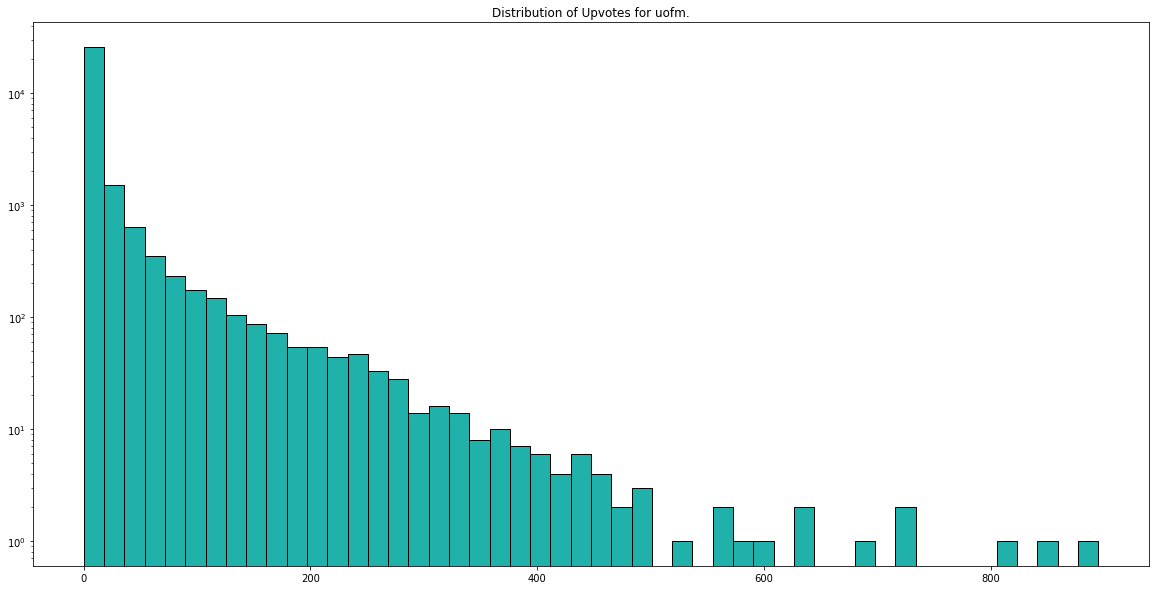
\includegraphics[width=\textwidth]{uofm_upvotes.png}
        \caption{Distribution of net upvote count for r/uofm.}
    \end{figure*}

    \begin{figure*}[!htb]
        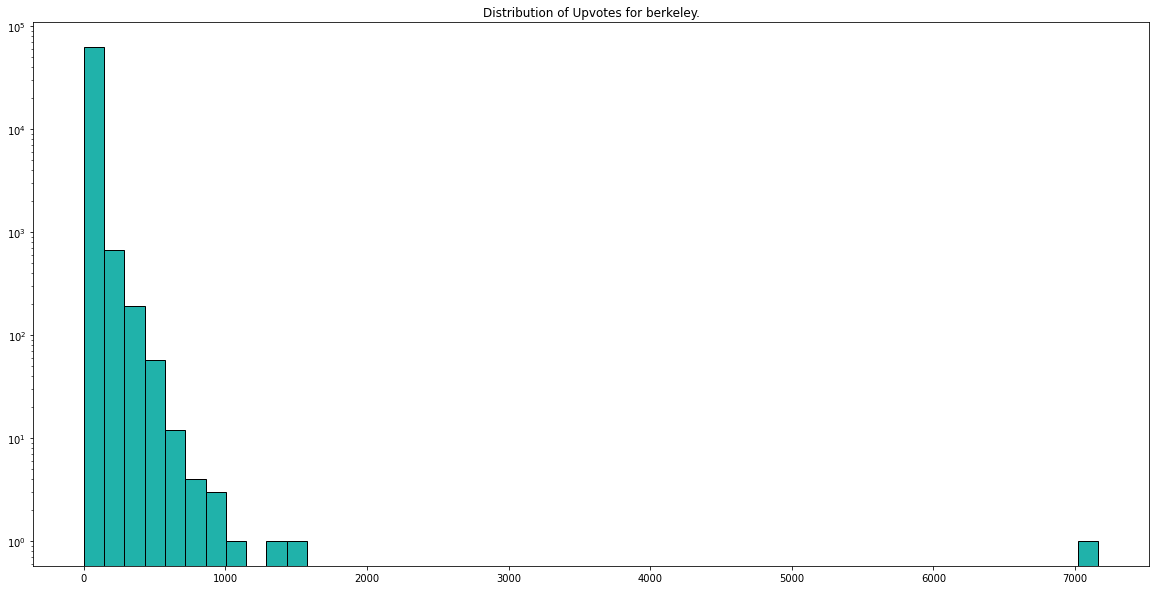
\includegraphics[width=\textwidth]{berkeley_upvotes.png}
        \caption{Distribution of net upvote count for r/berkeley.}
    \end{figure*}

    \begin{figure*}[!htb]
        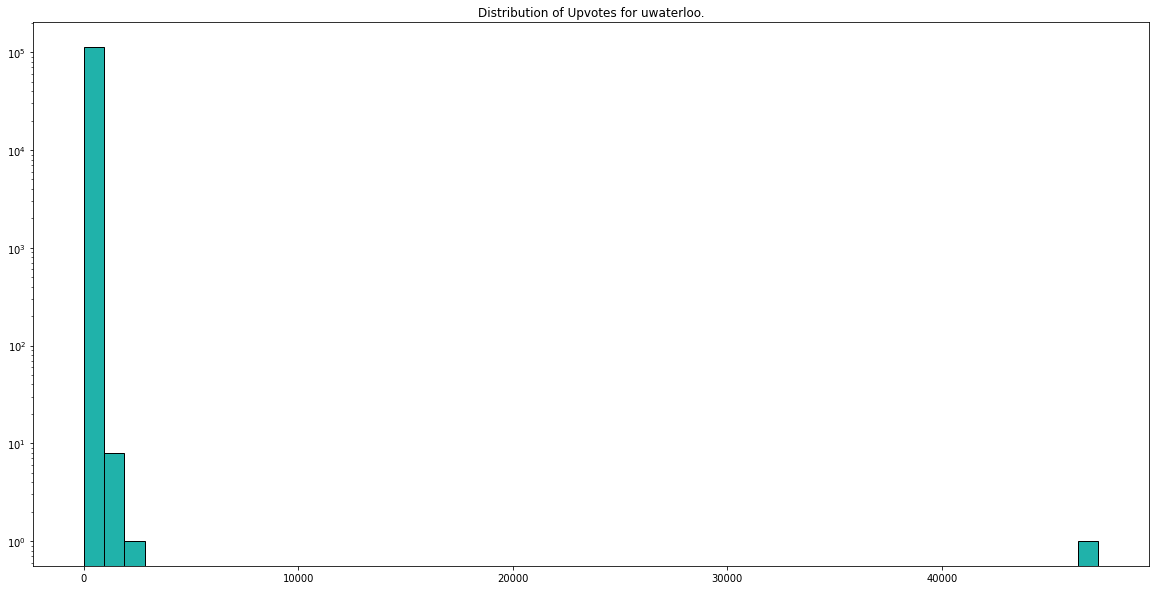
\includegraphics[width=\textwidth]{uwaterloo_upvotes.png}
        \caption{Distribution of net upvote count for r/uwaterloo.}
    \end{figure*}

    \begin{figure*}[!htb]
        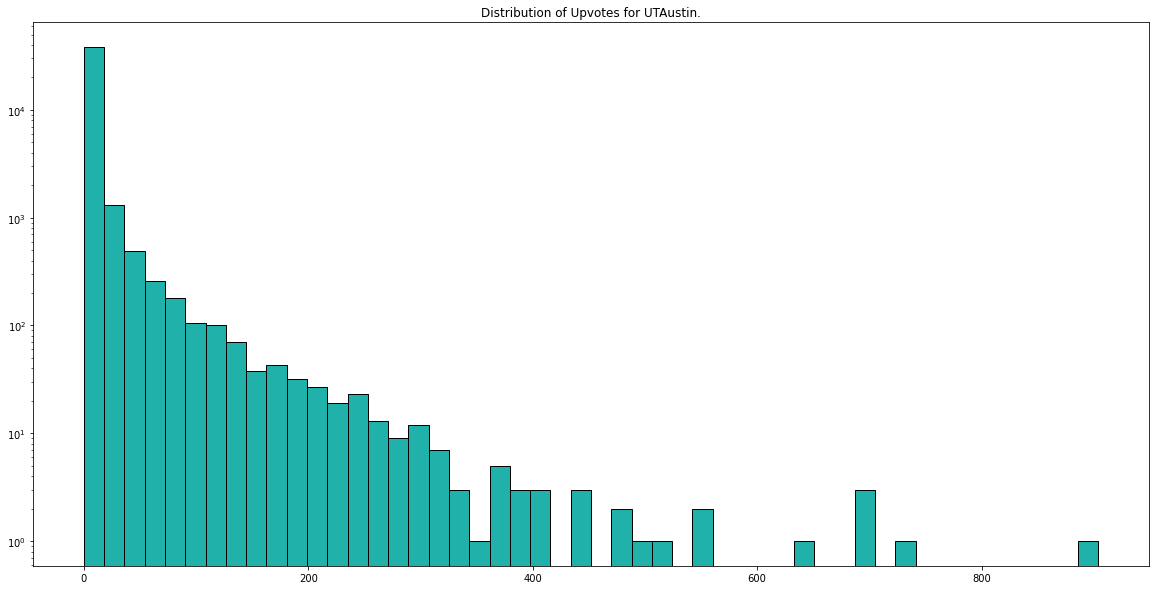
\includegraphics[width=\textwidth]{utaustin_upvotes.png}
        \caption{Distribution of net upvote count for r/UTAustin.}
    \end{figure*}

    \subsection{Histograms of upvote ratio for each subreddit after data cleaning and filtering.}
    \begin{figure*}
        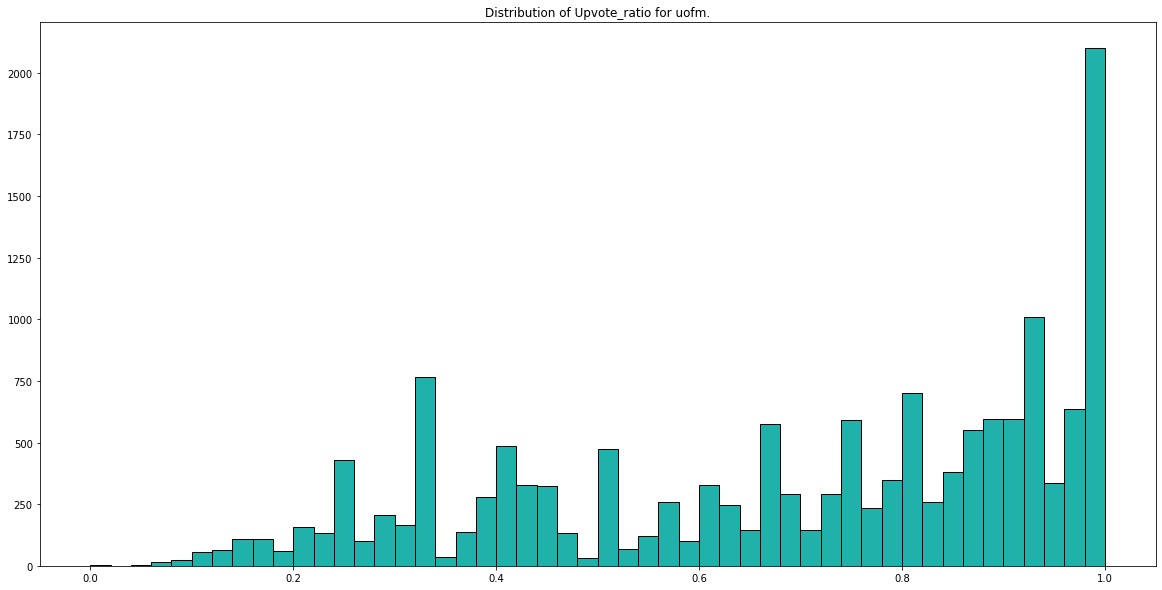
\includegraphics[width=\textwidth]{uofm_ratio1.png}
        \caption{Distribution of upvote ratio after data cleaning for r/uofm.}
    \end{figure*}
    \begin{figure*}
        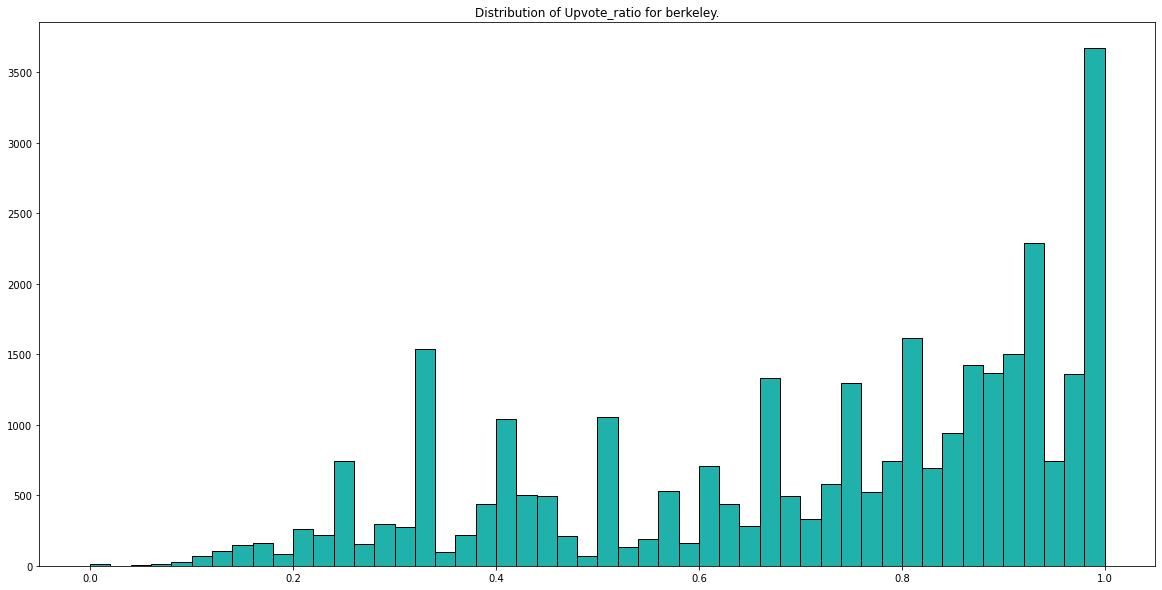
\includegraphics[width=\textwidth]{berkeley_ratio1.png}
        \caption{Distribution of upvote ratio after data cleaning for r/berkeley.}
    \end{figure*}
    \begin{figure*}
        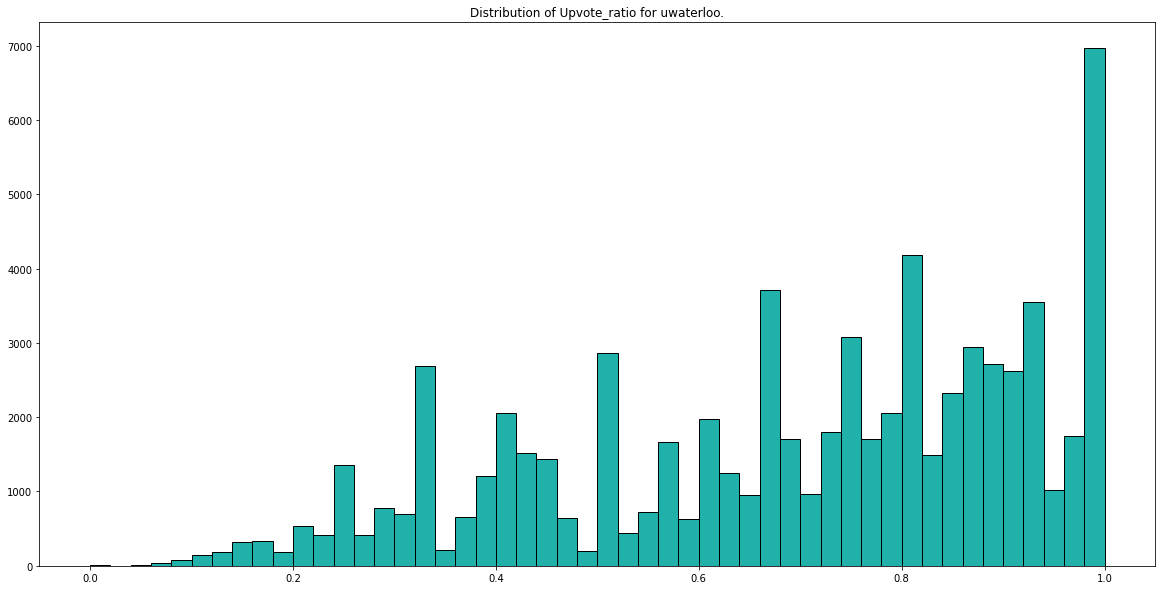
\includegraphics[width=\textwidth]{uwaterloo_ratio1.png}
        \caption{Distribution of upvote ratio after data cleaning for r/uwaterloo.}
    \end{figure*}
    \begin{figure*}
        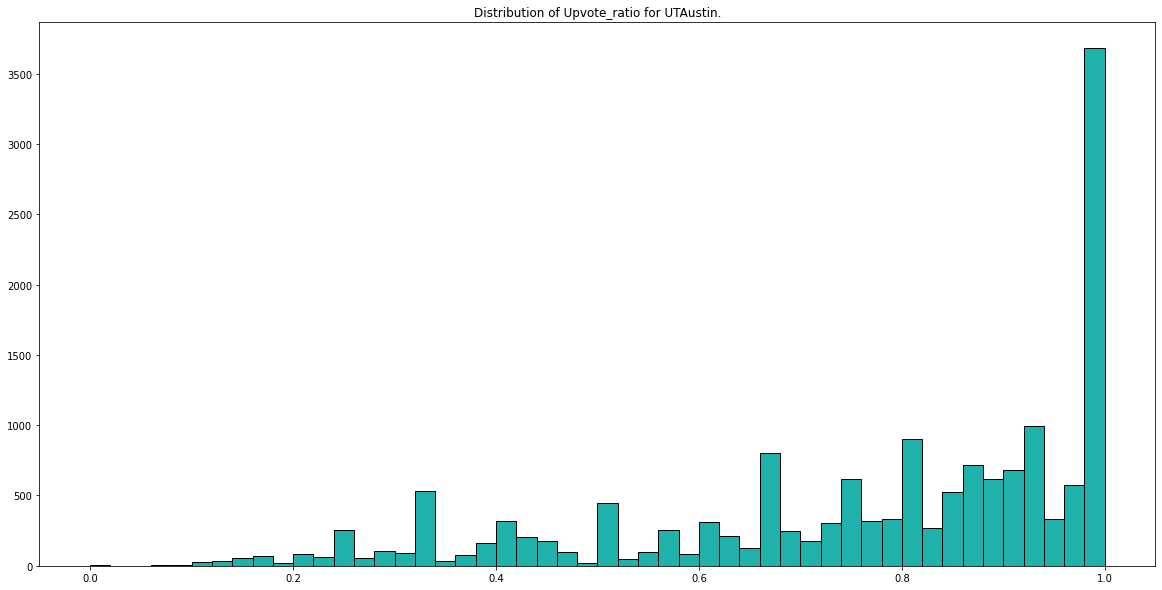
\includegraphics[width=\textwidth]{utaustin_ratio1.png}
        \caption{Distribution of upvote ratio after data cleaning for r/UTAustin.}
    \end{figure*}


    \subsection{Distribution of predicted upvote ratios using WMAE loss function.}
    \label{sec:appdistr}

    Below are the visualizations of both the true and predicted labels (upvote ratio) discussed in task 2 - the regression of upvote ratio. For each subreddit we include four histograms - the first (top left) displays the original distribution of upvote ratio in the test set after data filtering and removing posts with less than and including 20 total votes. The next figure (top right) shows the distribution of predicted upvote ratios on the test set by the neural network model trained using the MAE loss. The third figure (bottom left) shows the distribution of true upvote ratios after smoothing, with a fitted probability density curve. Finally, the fourth figure (bottom right) shows the distribution of predicted upvote ratios using the neural network model trained on the WMAE loss.

    \begin{figure}
        \begin{minipage}{0.5\textwidth}
            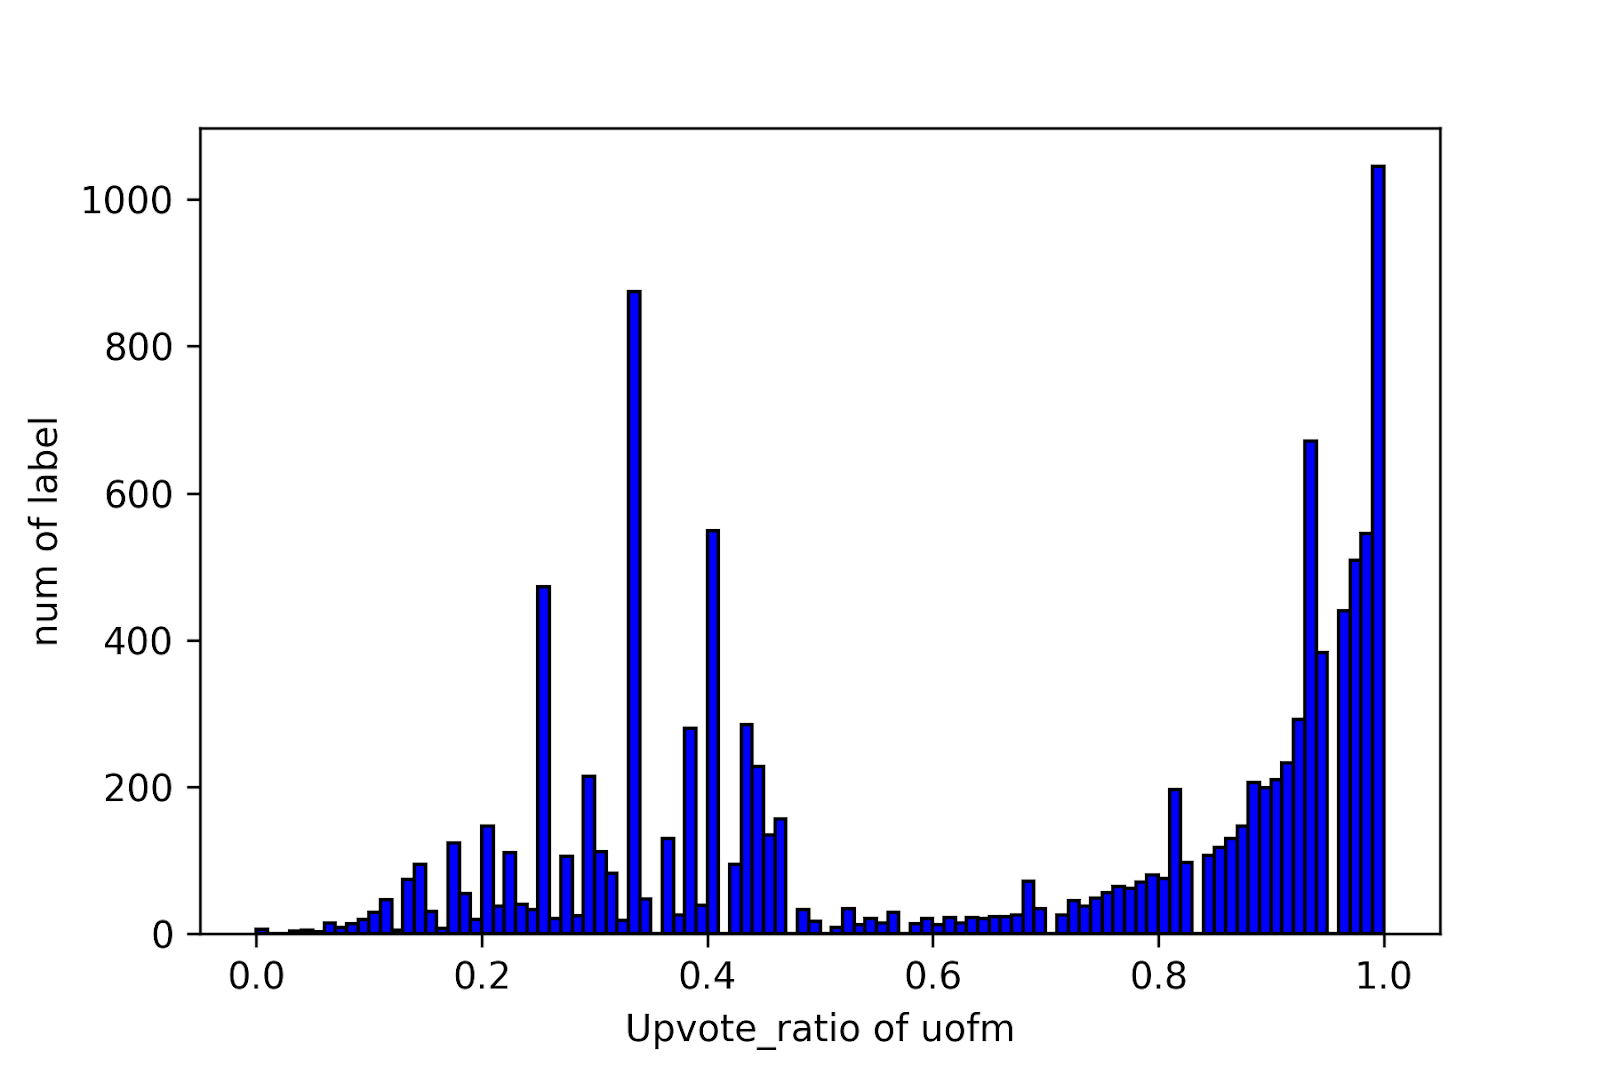
\includegraphics[width=\textwidth]{uofm_task2true_nonsmooth.png}
        \end{minipage}
        \begin{minipage}{0.5\textwidth}
            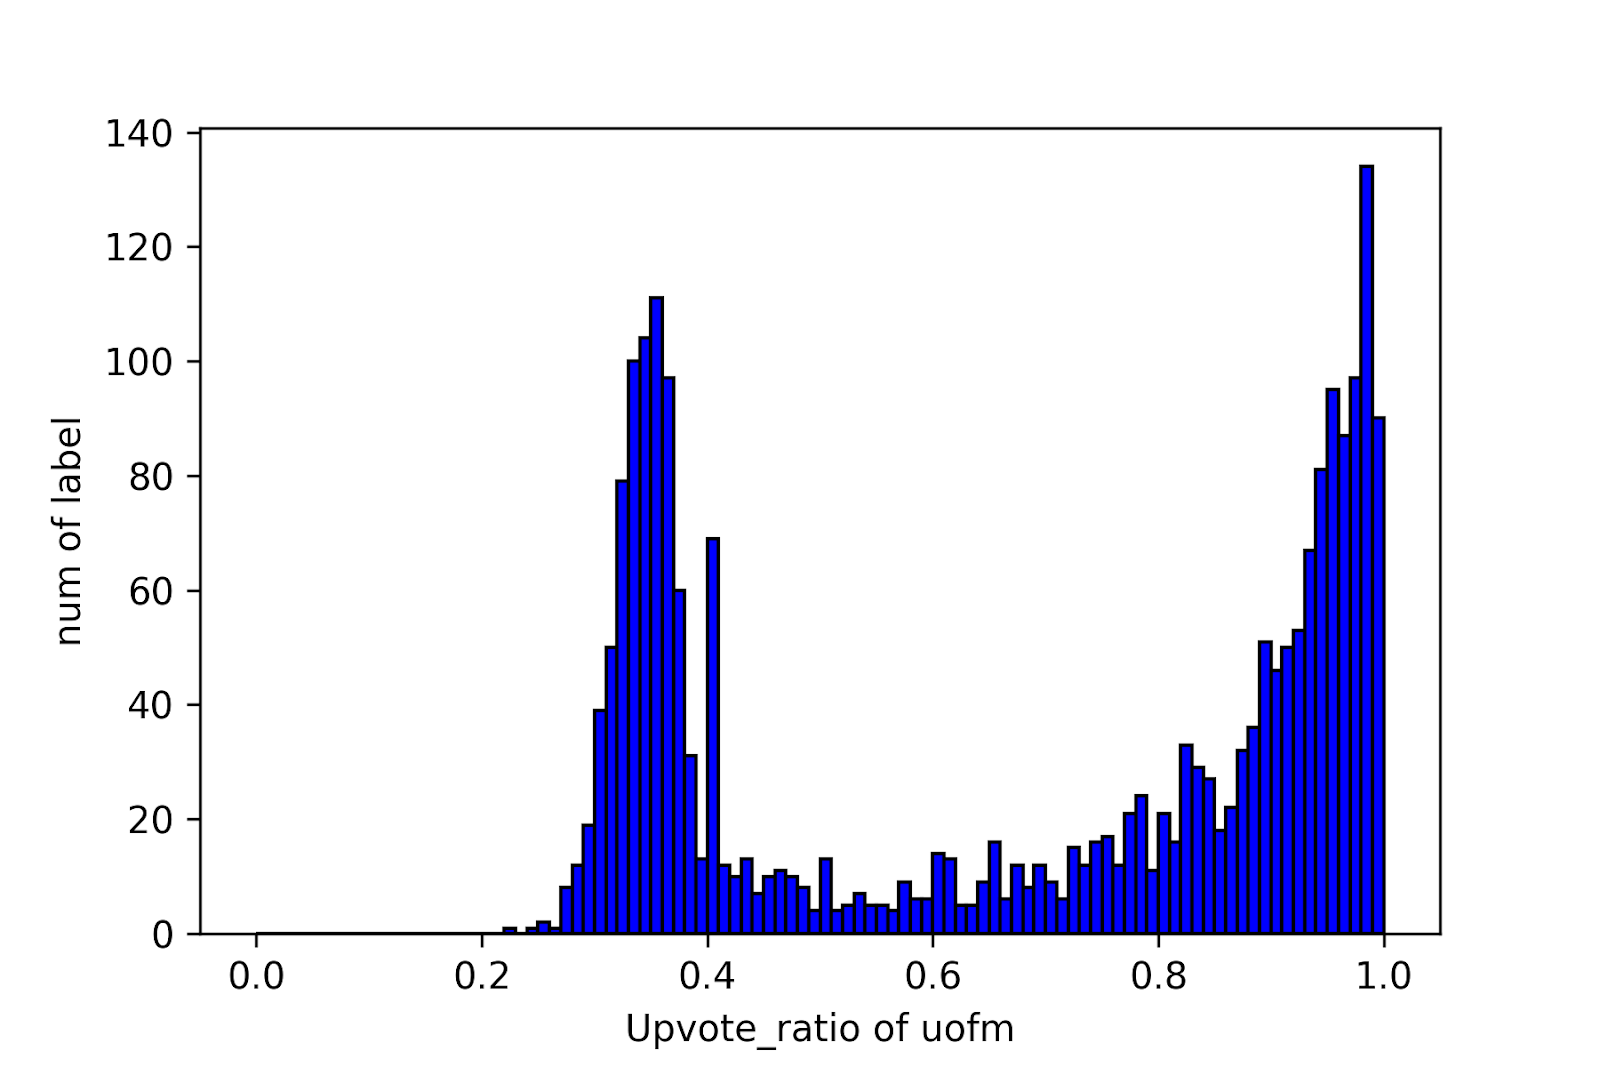
\includegraphics[width=\textwidth]{uofm_task2pred_nonsmooth.png}
        \end{minipage}

        \begin{minipage}{0.5\textwidth}
            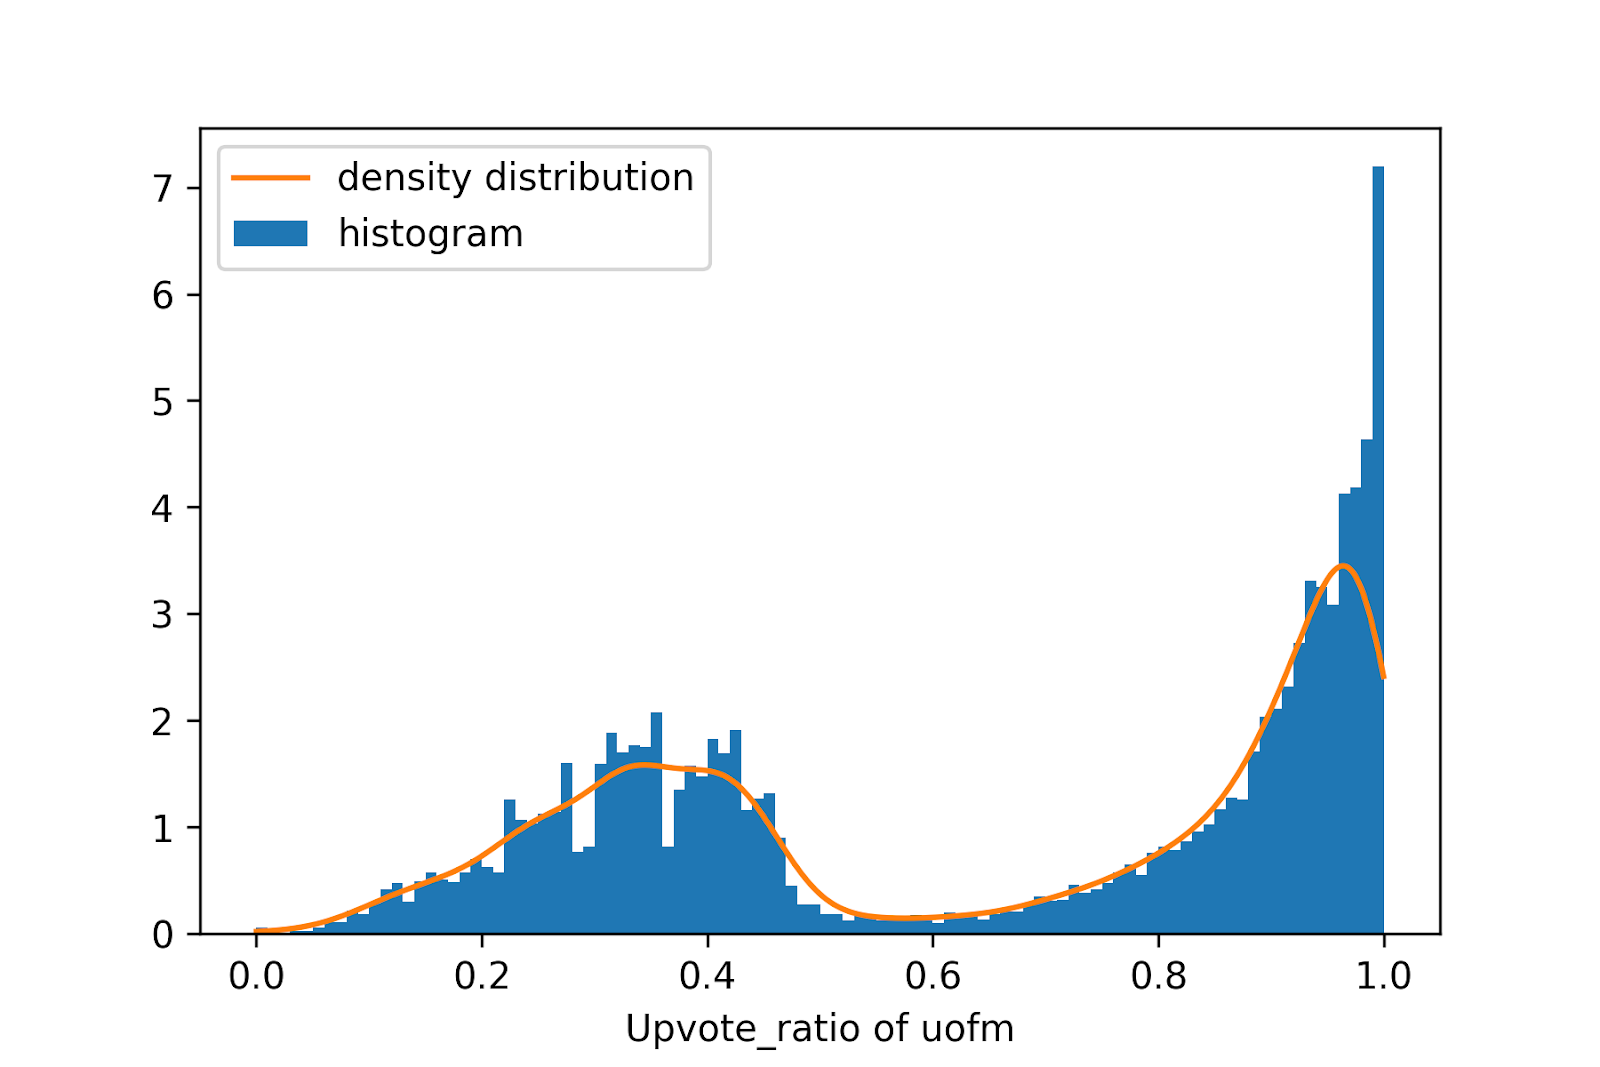
\includegraphics[width=\textwidth]{uofm_task2true_smooth.png}
        \end{minipage}
        \begin{minipage}{0.5\textwidth}
            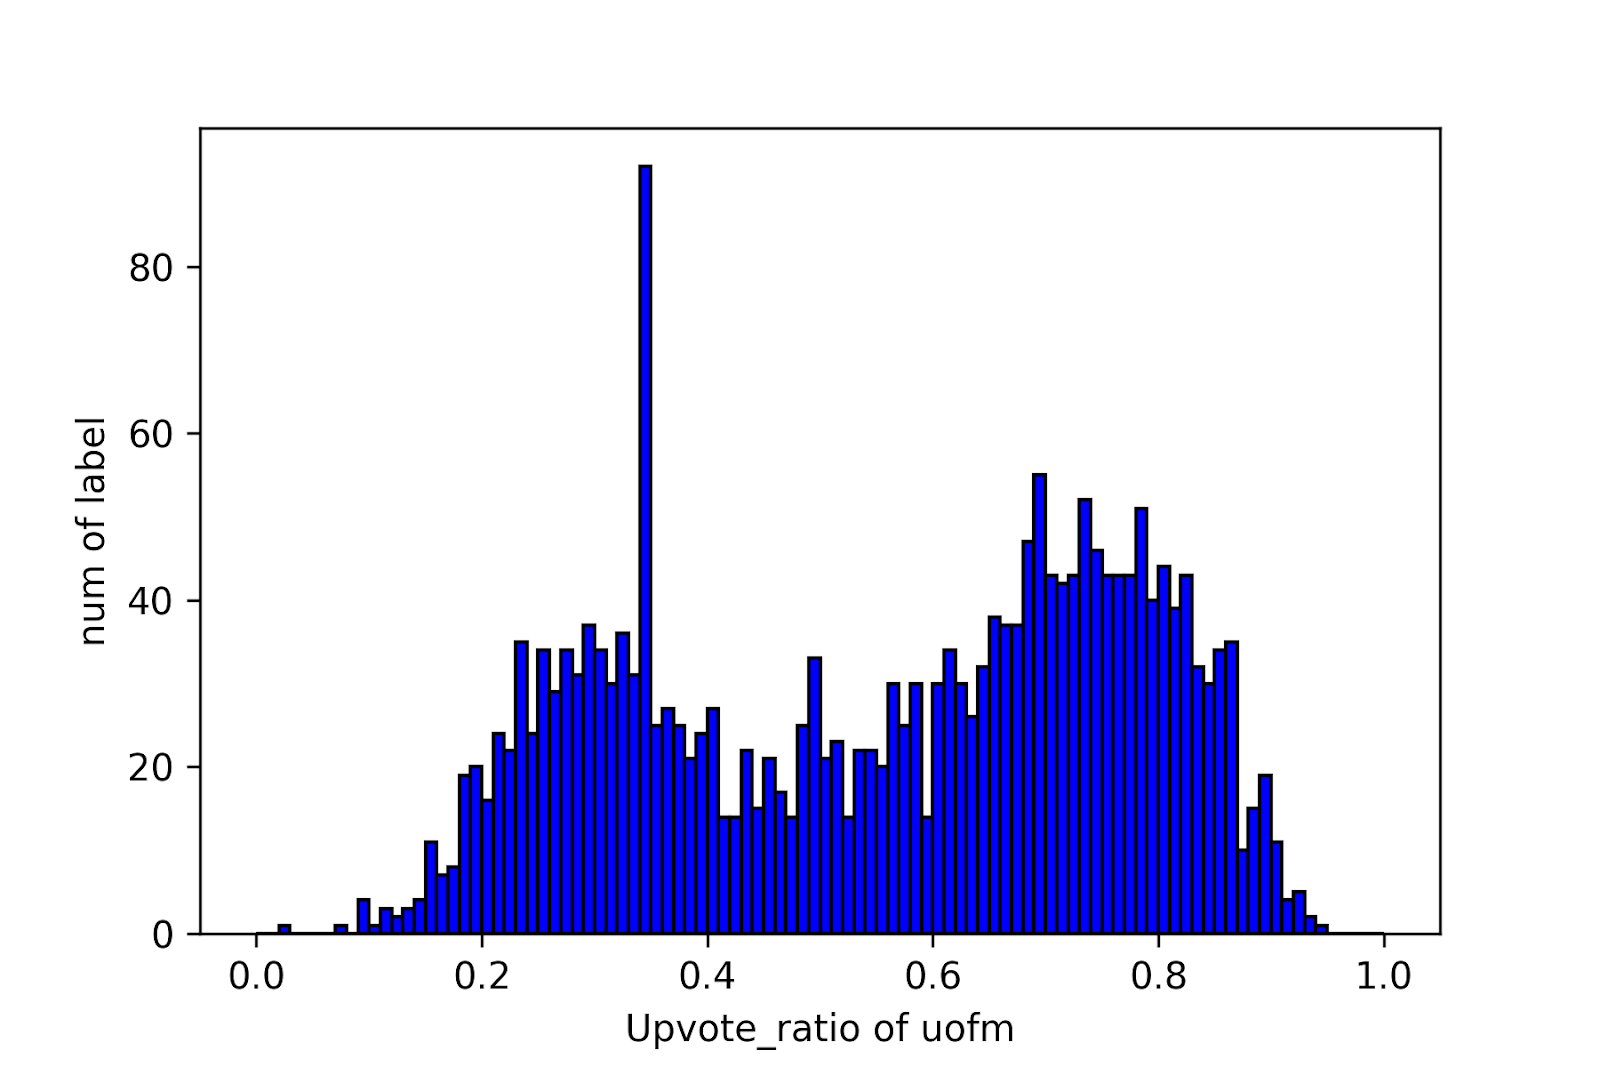
\includegraphics[width=\textwidth]{uofm_task2pred_smooth.png}
        \end{minipage}

        \caption{
            Top left - distribution of true upvote ratios for test set for r/uofm.
            Top right - distribution of predicted labels of test set using neural network trained on MAE loss for r/uofm.
            Bottom left - distribution of true upvote ratios for test set after smoothing and fitted density function for r/uofm.
            Bottom right - distribution of predicted labels of test set using neural network trained on WMAE loss for r/uofm.
        }
    \end{figure}

    \begin{figure}
        \begin{minipage}{0.5\textwidth}
            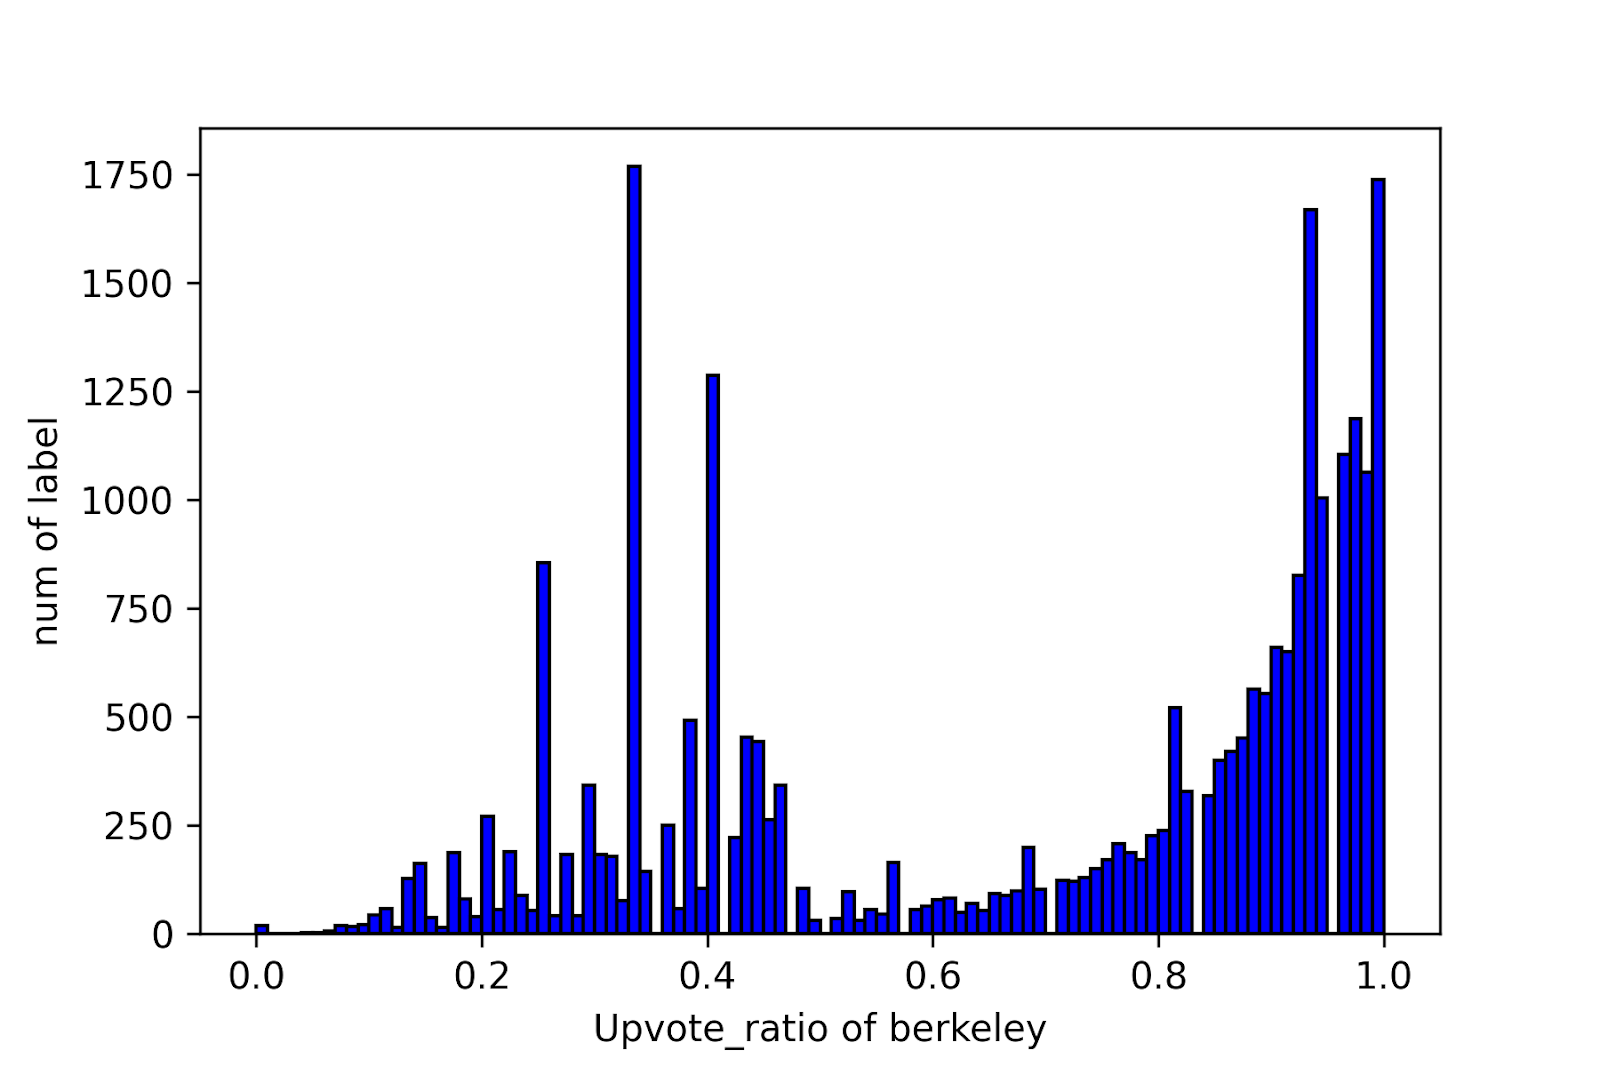
\includegraphics[width=\textwidth]{berkeley_task2true_nonsmooth.png}
        \end{minipage}
        \begin{minipage}{0.5\textwidth}
            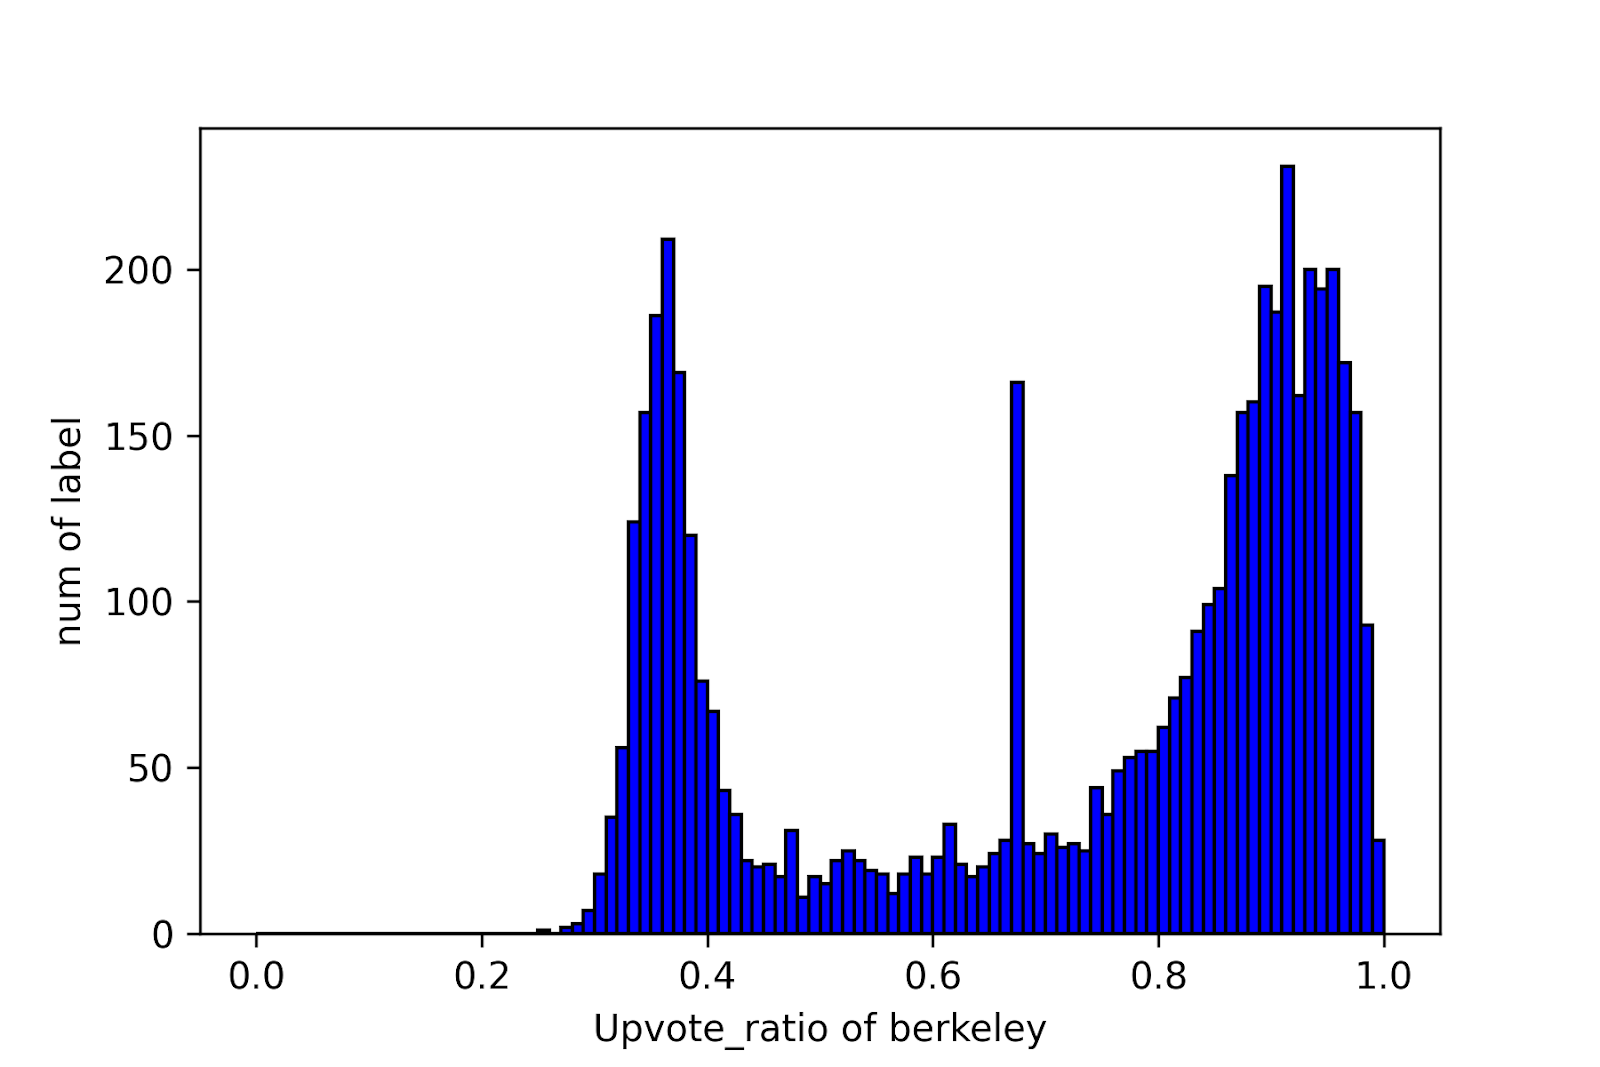
\includegraphics[width=\textwidth]{berkeley_task2pred_nonsmooth.png}
        \end{minipage}

        \begin{minipage}{0.5\textwidth}
            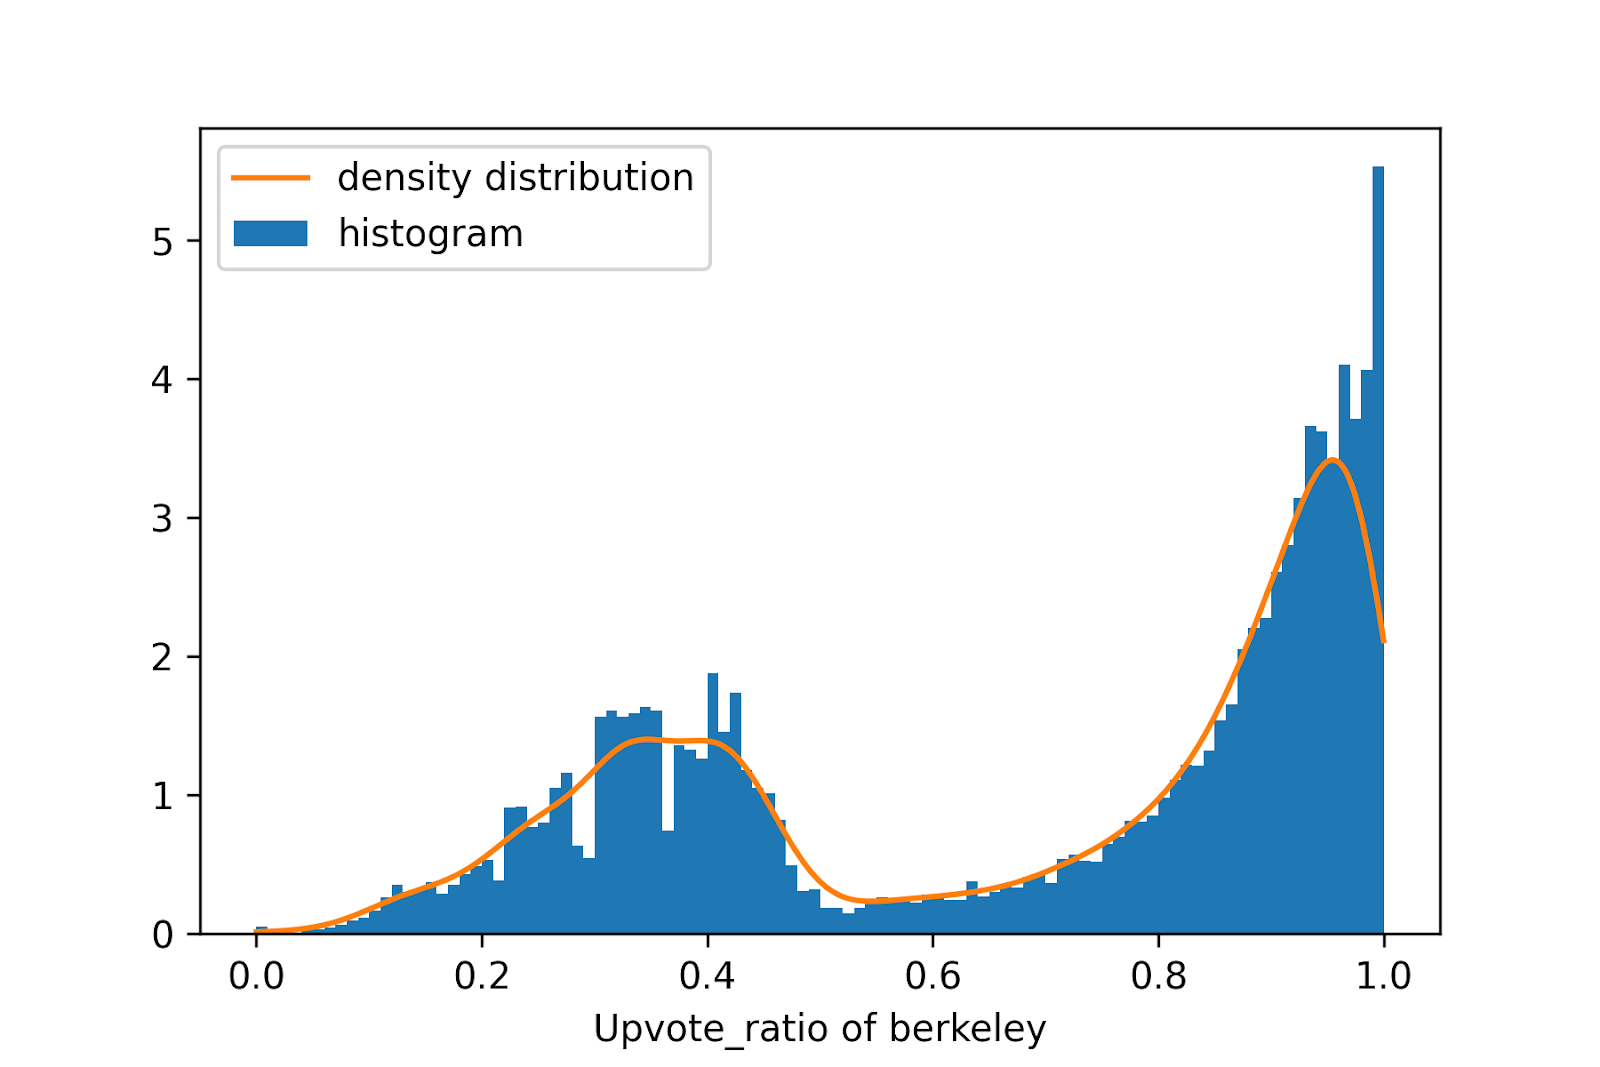
\includegraphics[width=\textwidth]{berkeley_task2true_smooth.png}
        \end{minipage}
        \begin{minipage}{0.5\textwidth}
            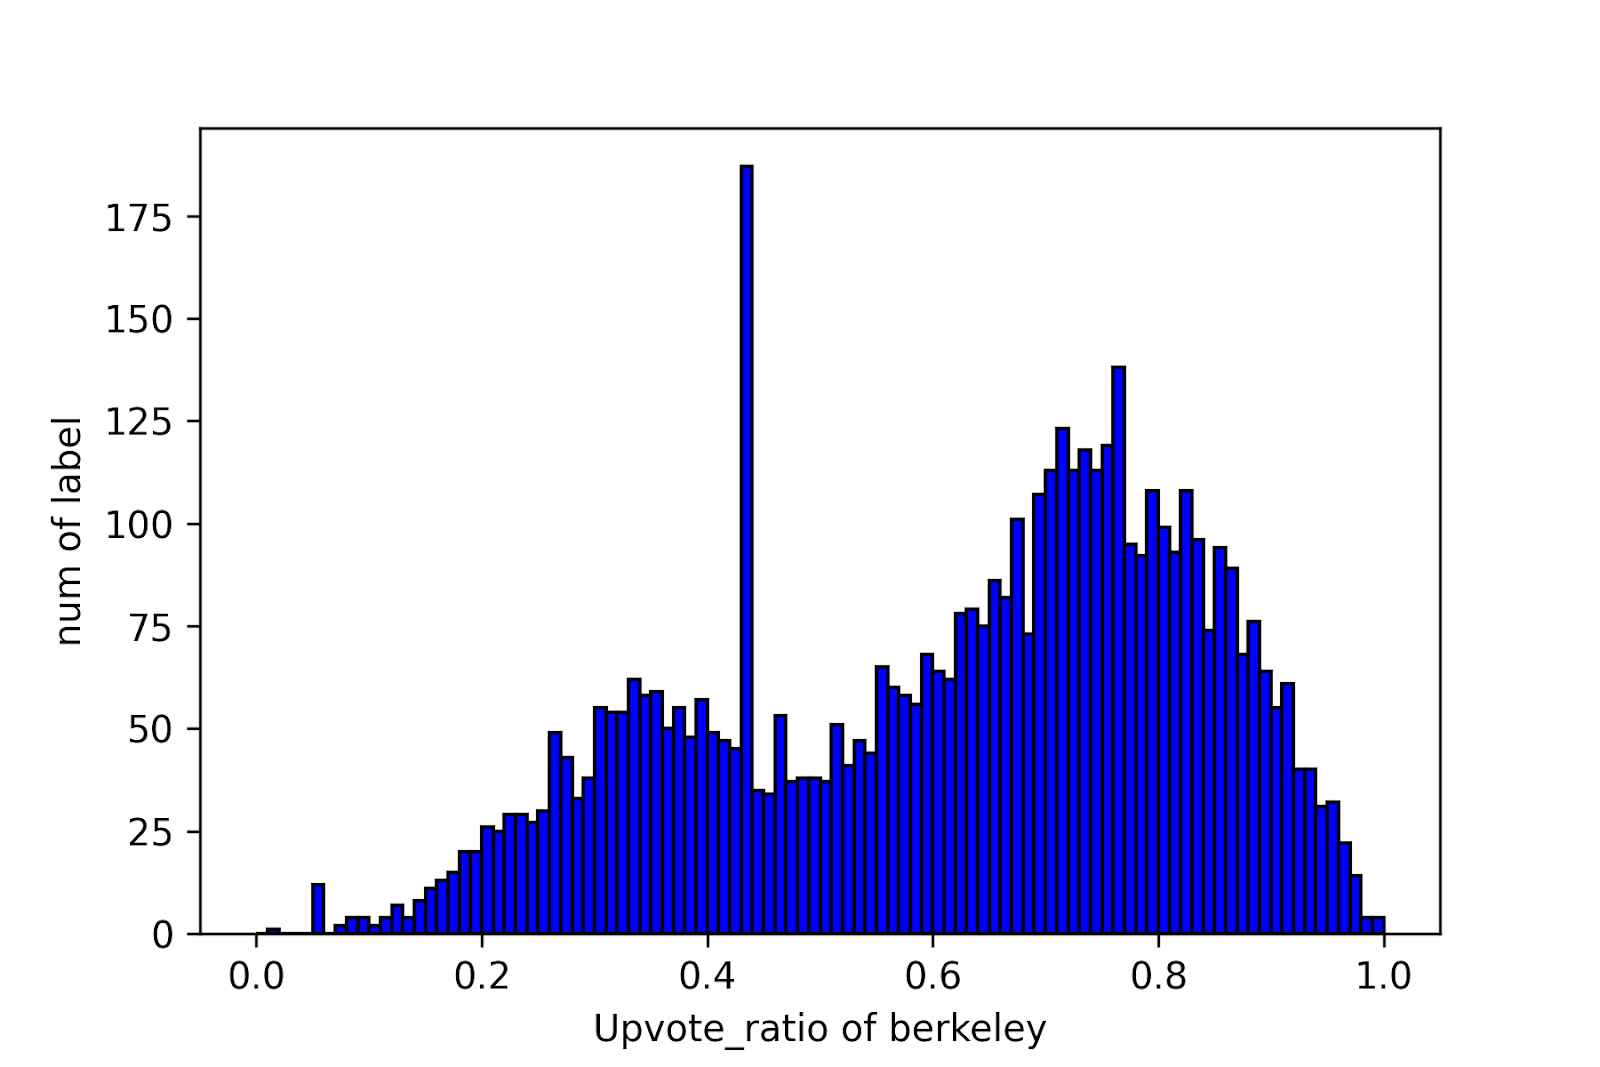
\includegraphics[width=\textwidth]{berkeley_task2pred_smooth.png}
        \end{minipage}

        \caption{
            Top left - distribution of true upvote ratios for test set for r/berkeley.
            Top right - distribution of predicted labels of test set using neural network trained on MAE loss for r/berkeley.
            Bottom left - distribution of true upvote ratios for test set after smoothing and fitted density function for r/berkeley.
            Bottom right - distribution of predicted labels of test set using neural network trained on WMAE loss for r/berkeley.
        }
    \end{figure}

    \begin{figure}
        \begin{minipage}{0.5\textwidth}
            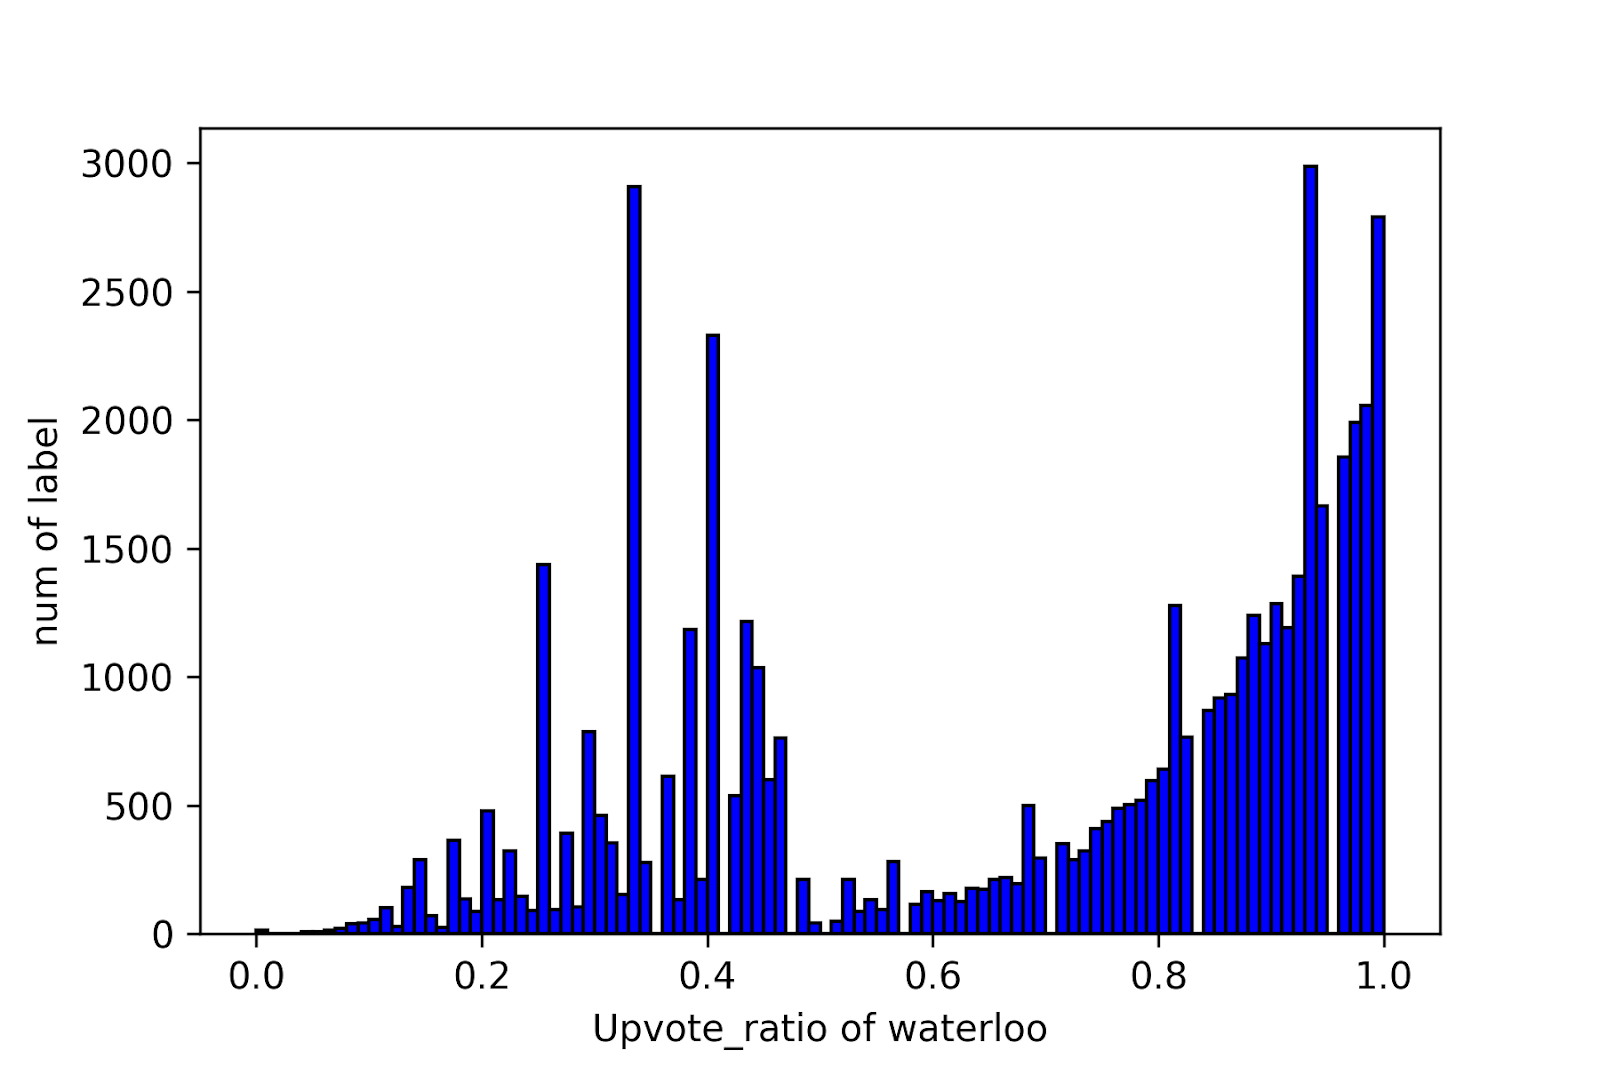
\includegraphics[width=\textwidth]{uwaterloo_task2true_nonsmooth.png}
        \end{minipage}
        \begin{minipage}{0.5\textwidth}
            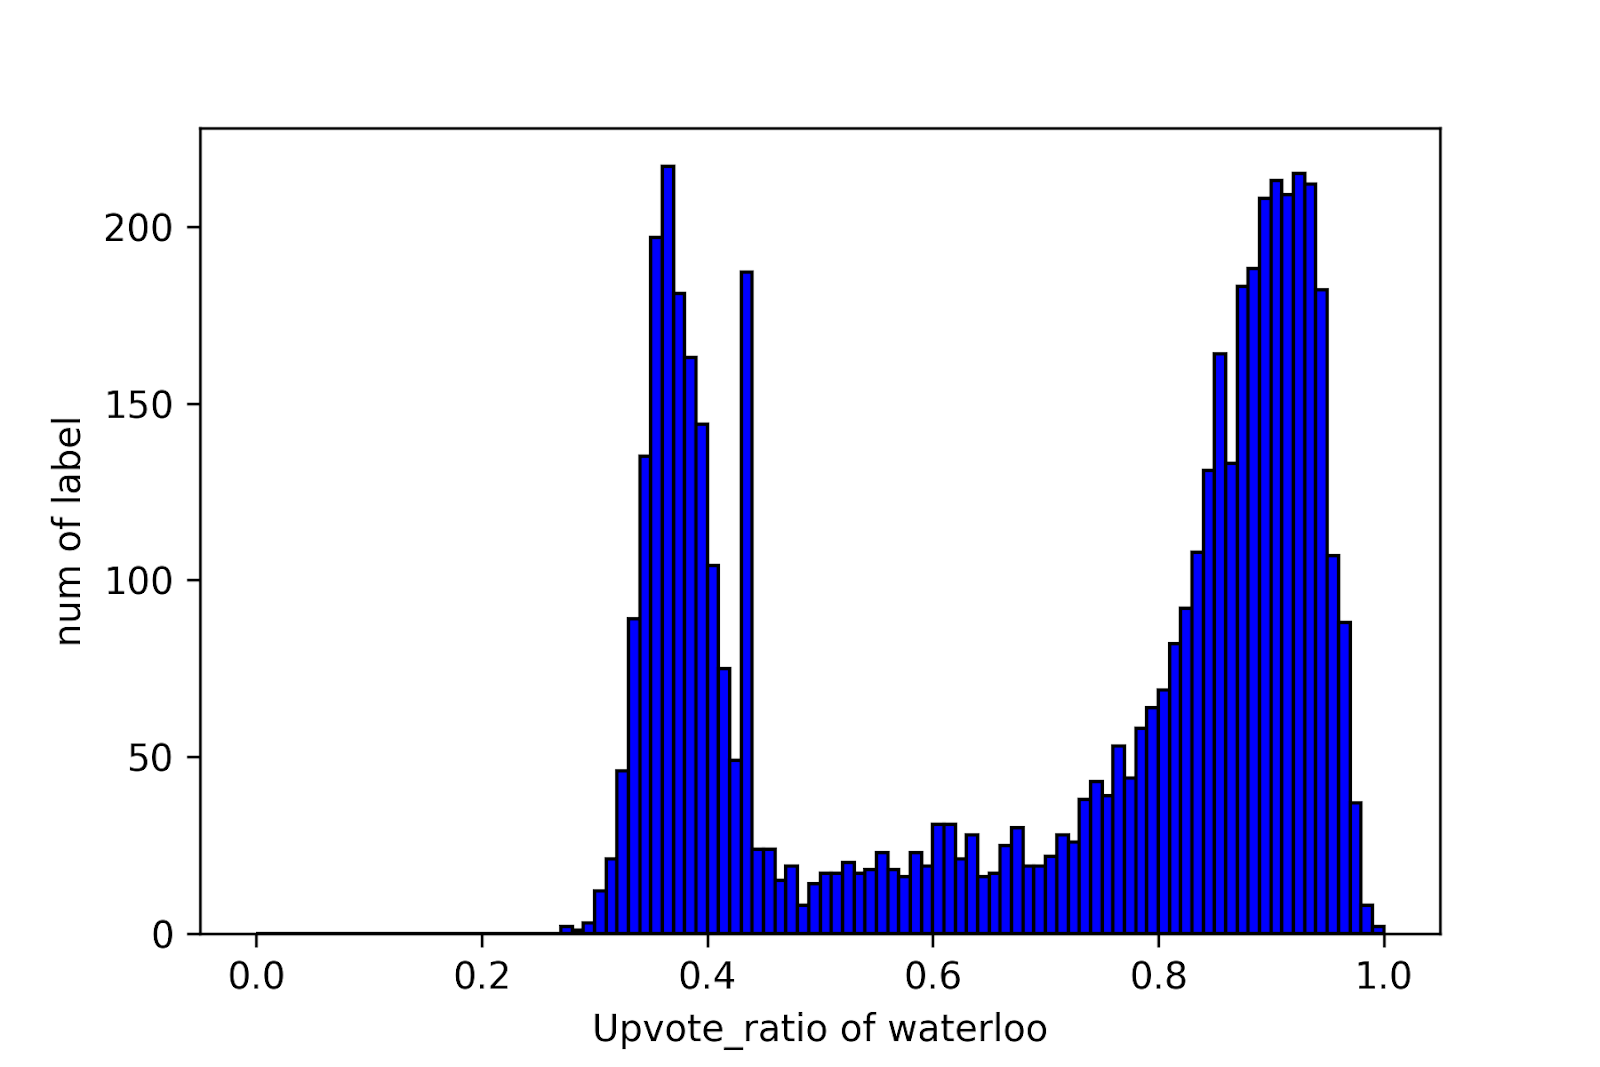
\includegraphics[width=\textwidth]{uwaterloo_task2pred_nonsmooth.png}
        \end{minipage}

        \begin{minipage}{0.5\textwidth}
            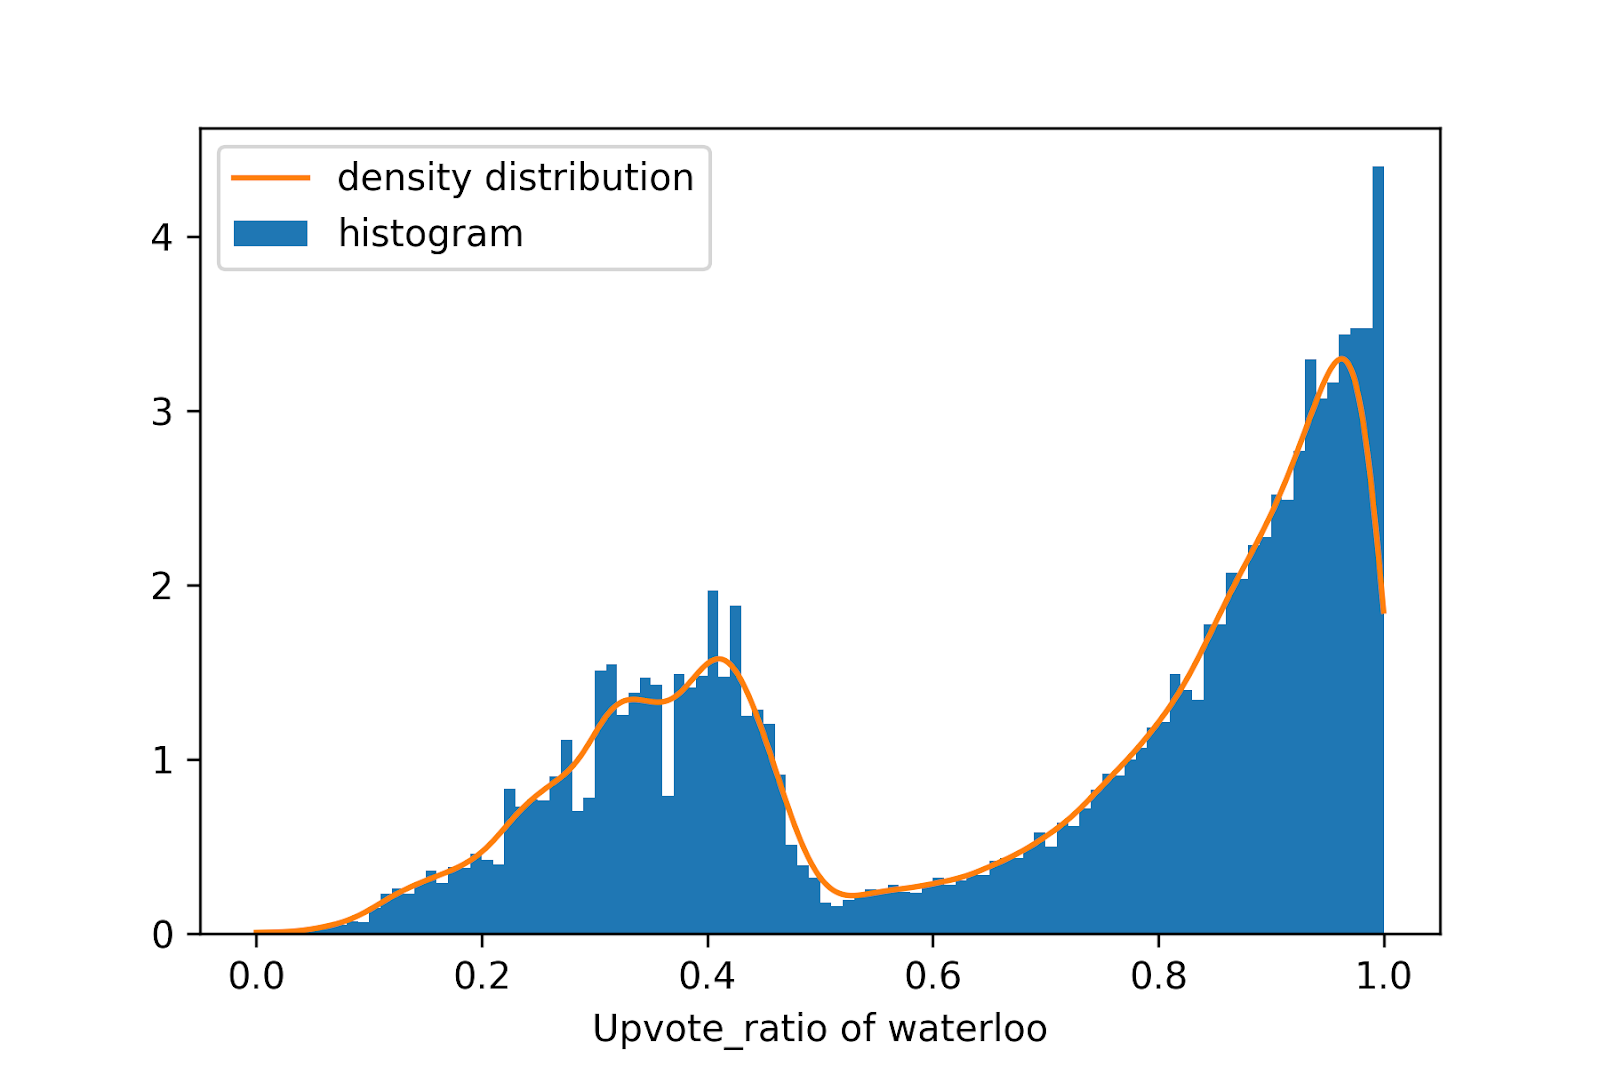
\includegraphics[width=\textwidth]{uwaterloo_task2true_smooth.png}
        \end{minipage}
        \begin{minipage}{0.5\textwidth}
            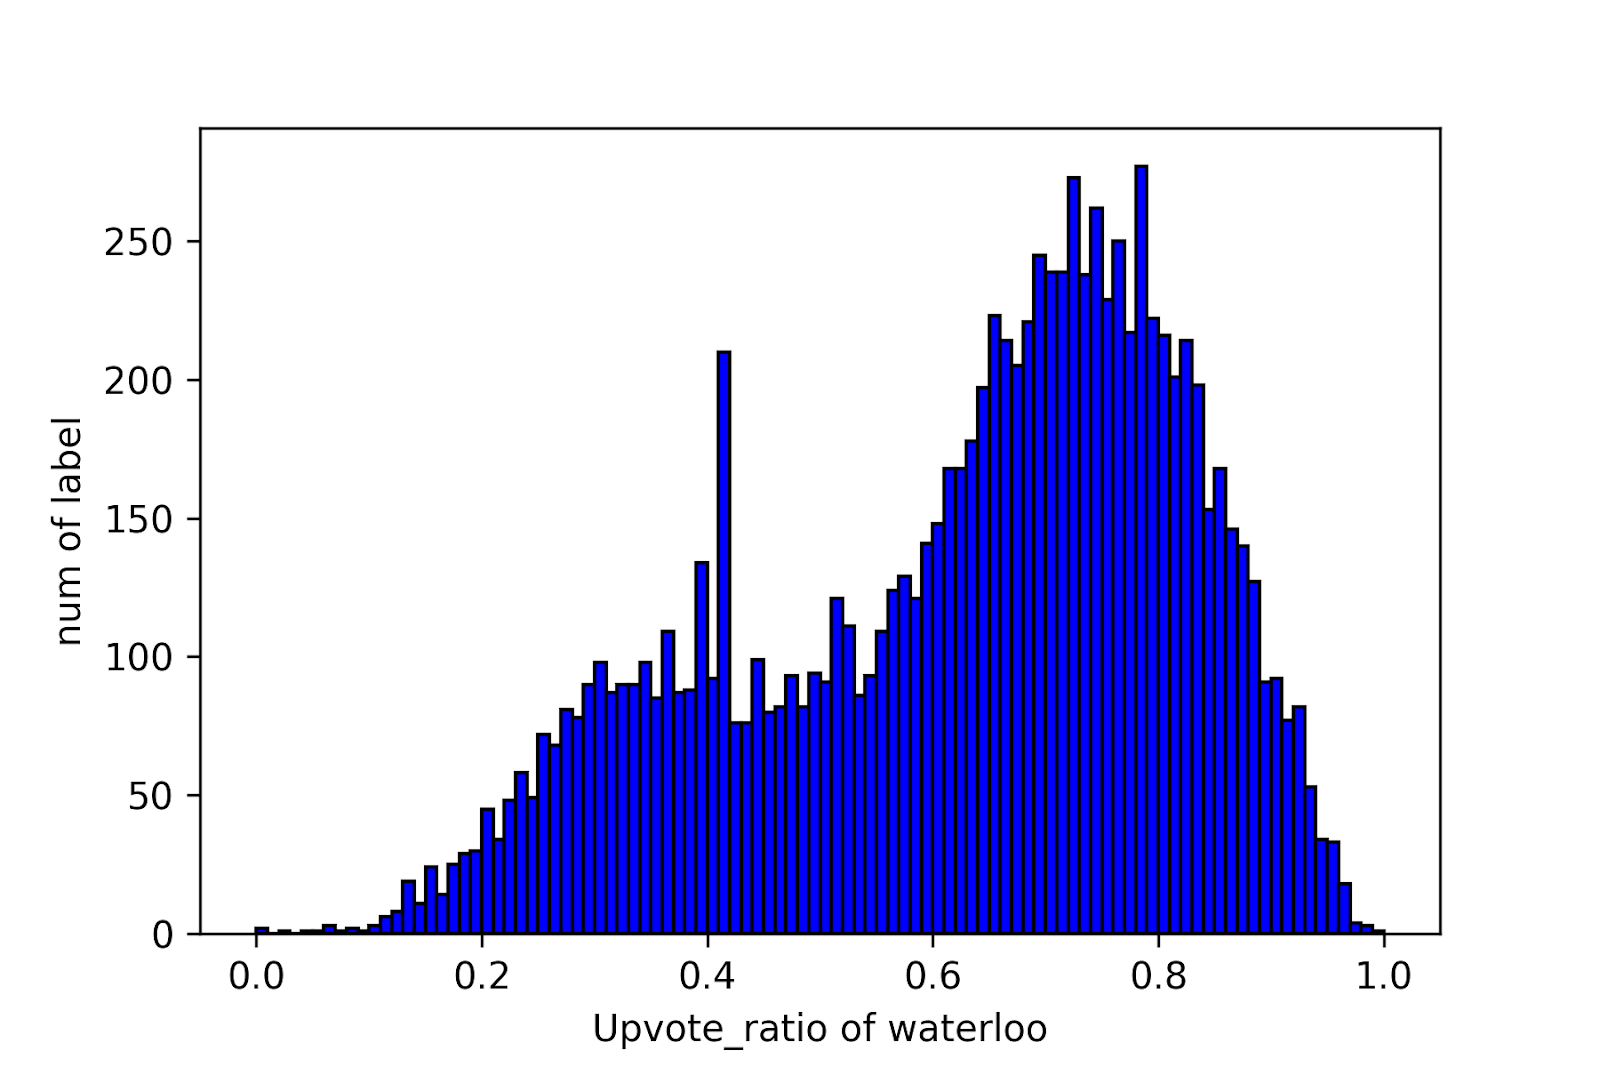
\includegraphics[width=\textwidth]{uwaterloo_task2pred_smooth.png}
        \end{minipage}

        \caption{
            Top left - distribution of true upvote ratios for test set for r/uwaterloo.
            Top right - distribution of predicted labels of test set using neural network trained on MAE loss for r/uwaterloo.
            Bottom left - distribution of true upvote ratios for test set after smoothing and fitted density function for r/uwaterloo.
            Bottom right - distribution of predicted labels of test set using neural network trained on WMAE loss for r/uwaterloo.
        }
    \end{figure}

    \begin{figure}
        \begin{minipage}{0.5\textwidth}
            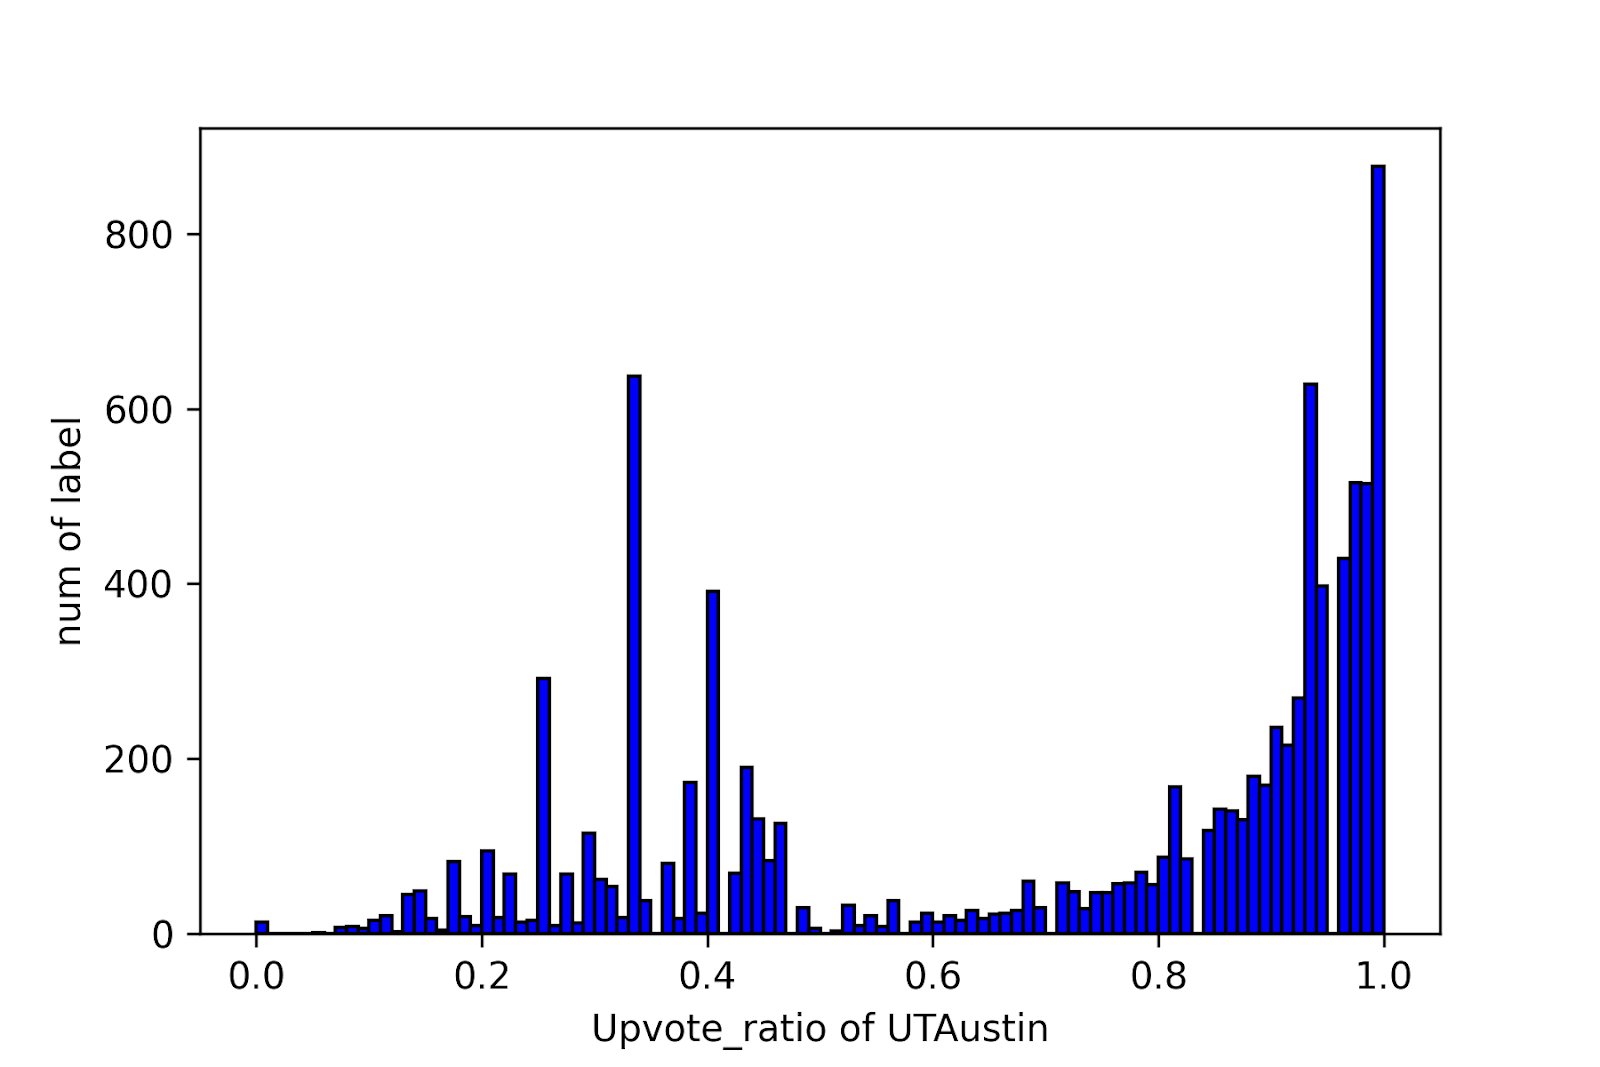
\includegraphics[width=\textwidth]{utaustin_task2true_nonsmooth.png}
        \end{minipage}
        \begin{minipage}{0.5\textwidth}
            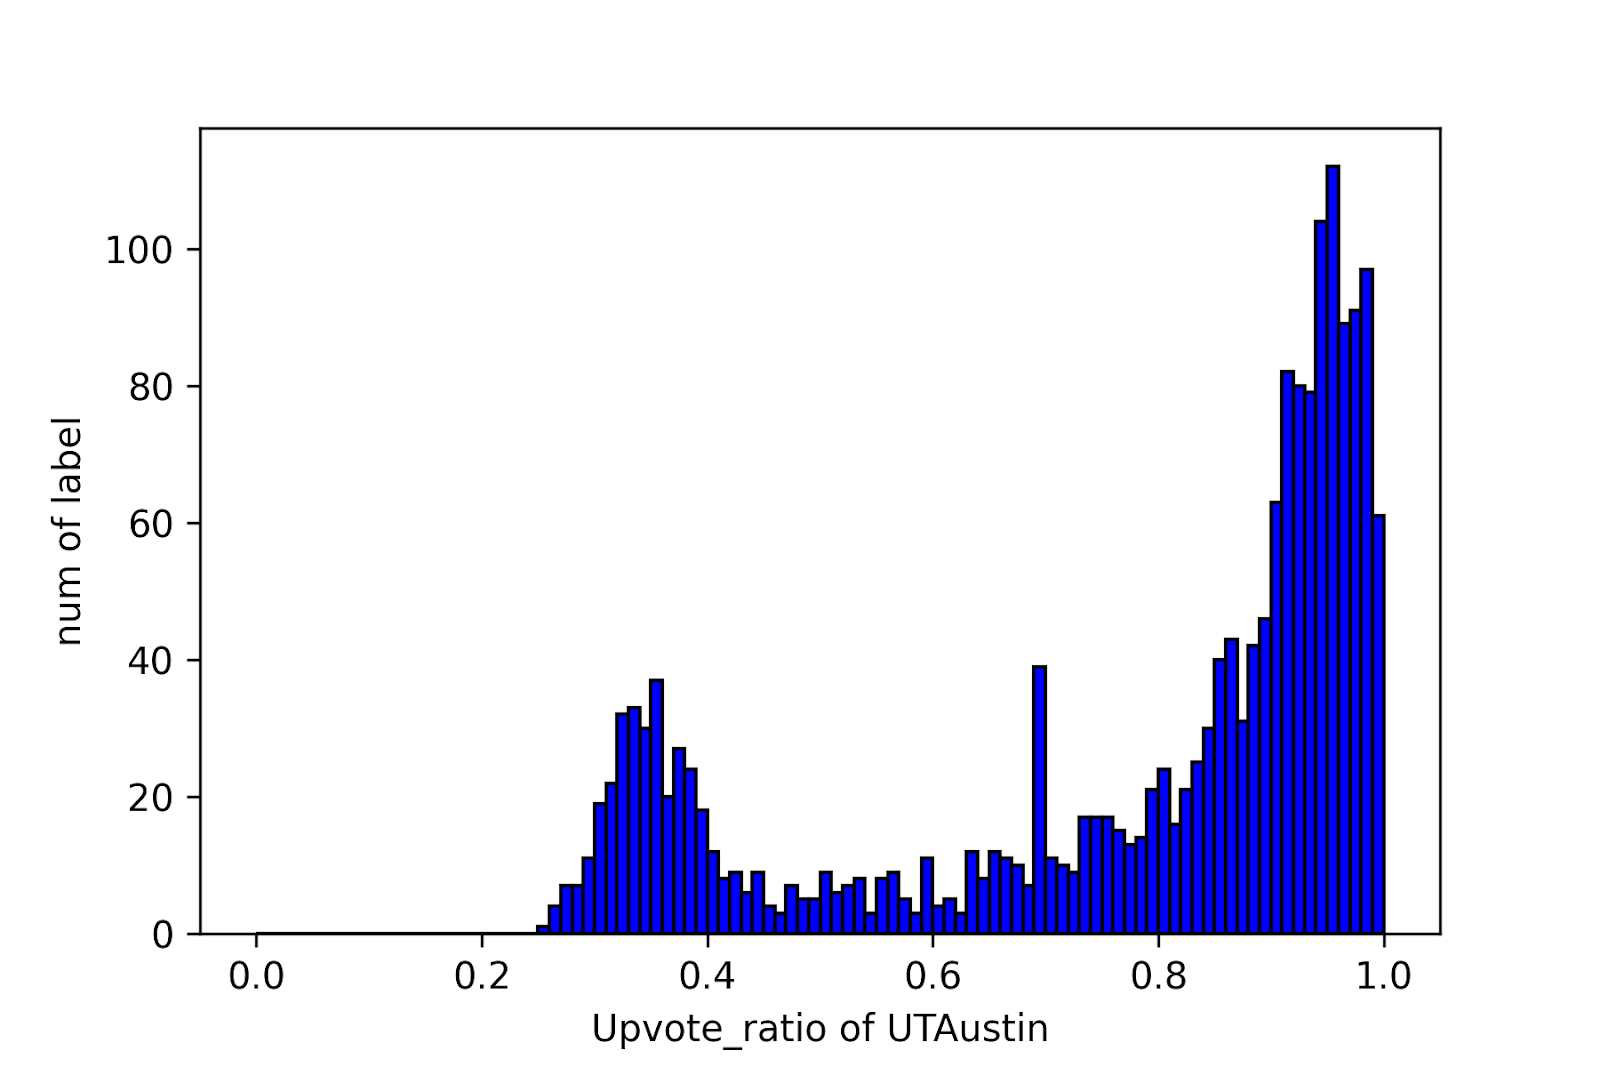
\includegraphics[width=\textwidth]{utaustin_task2pred_nonsmooth.png}
        \end{minipage}

        \begin{minipage}{0.5\textwidth}
            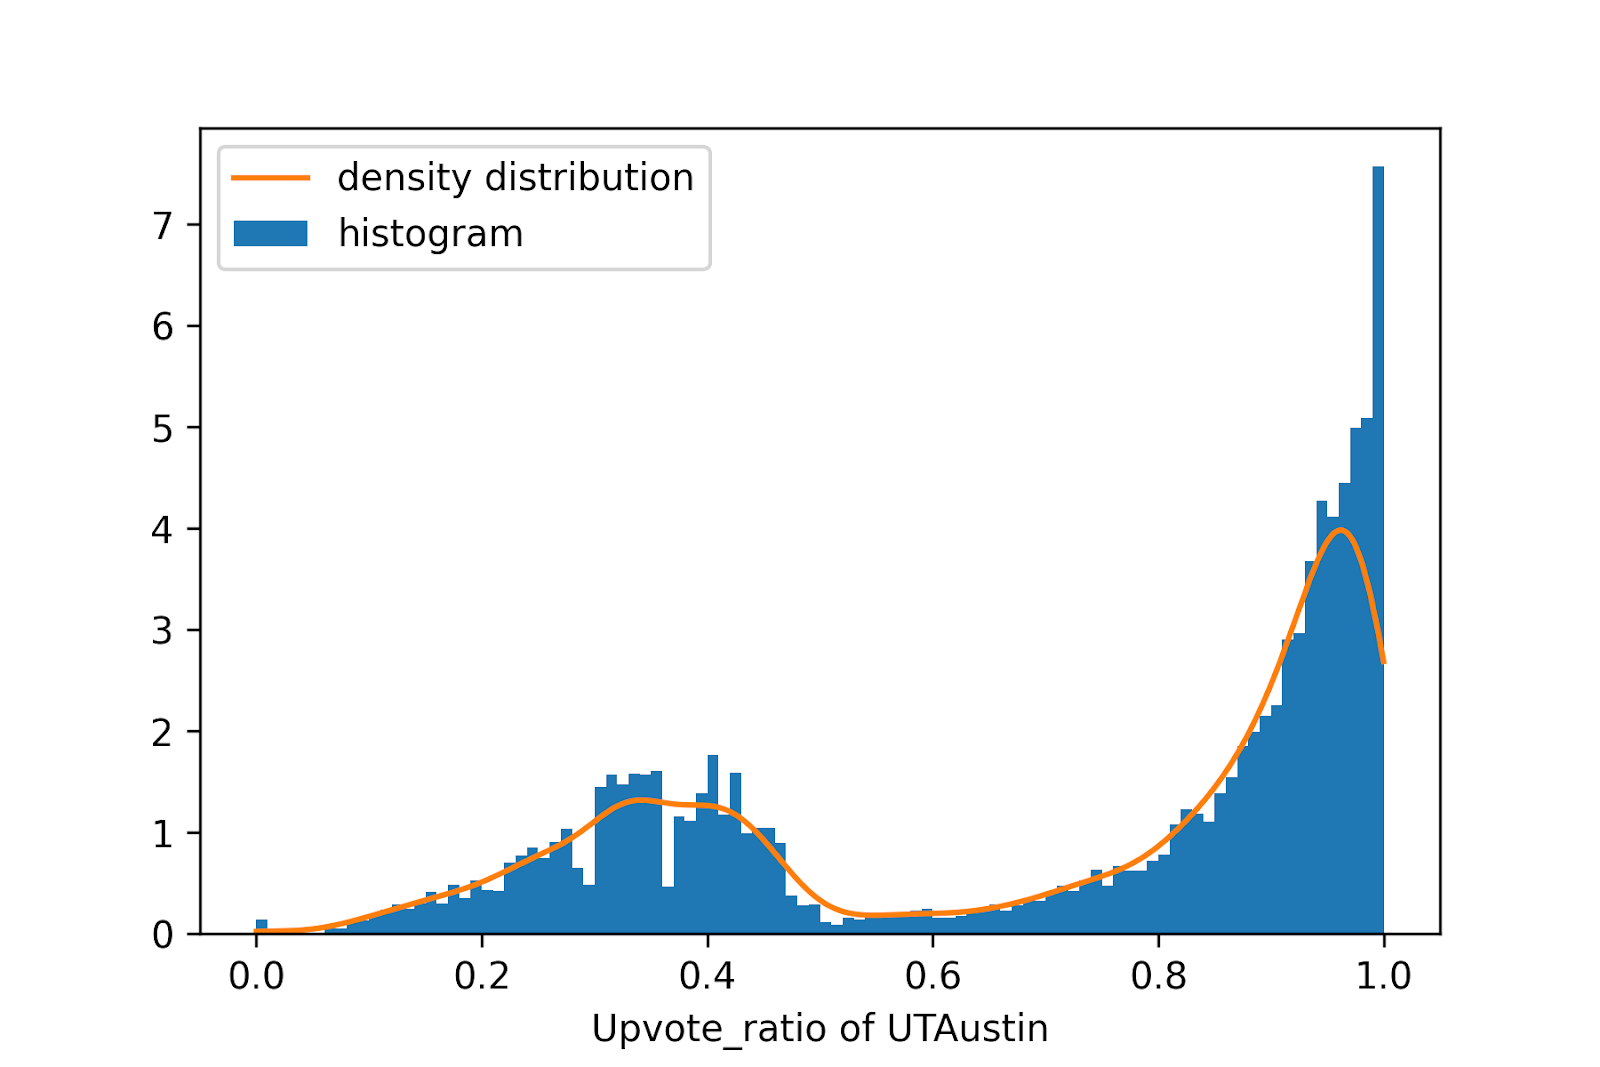
\includegraphics[width=\textwidth]{utaustin_task2true_smooth.png}
        \end{minipage}
        \begin{minipage}{0.5\textwidth}
            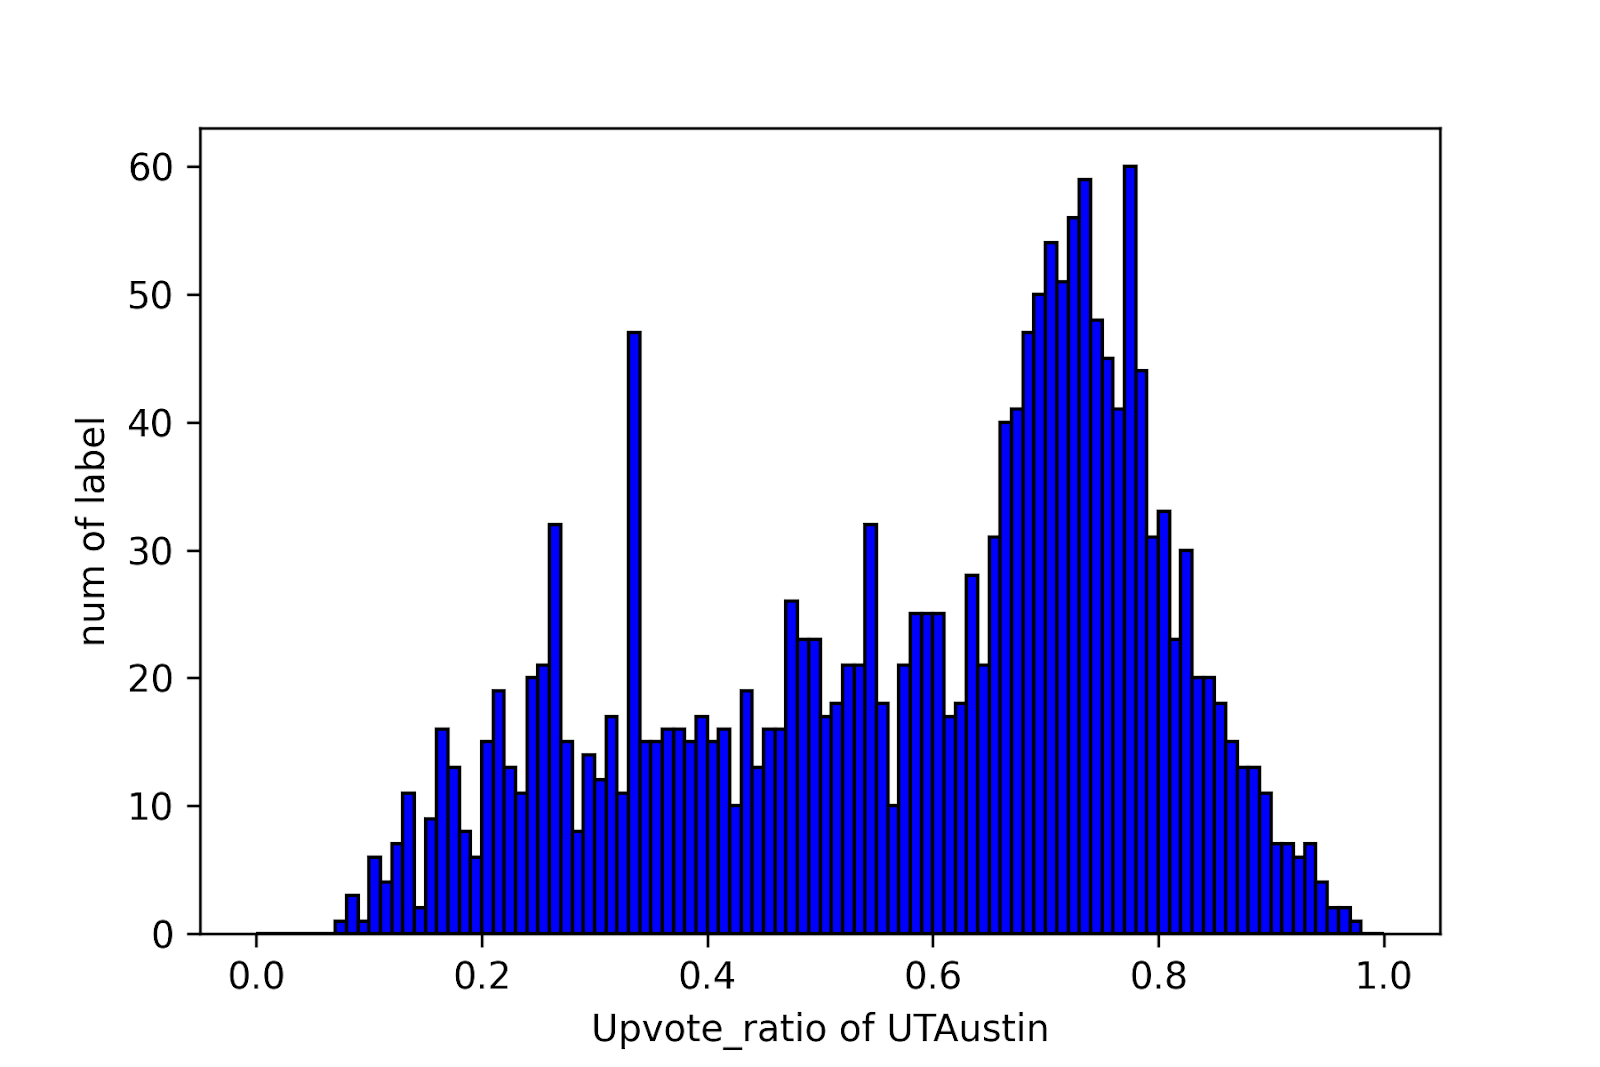
\includegraphics[width=\textwidth]{utaustin_task2pred_smooth.png}
        \end{minipage}

        \caption{
            Top left - distribution of true upvote ratios for test set for r/UTAustin.
            Top right - distribution of predicted labels of test set using neural network trained on MAE loss for r/UTAustin.
            Bottom left - distribution of true upvote ratios for test set after smoothing and fitted density function for r/UTAustin.
            Bottom right - distribution of predicted labels of test set using neural network trained on WMAE loss for r/UTAustin.
        }
    \end{figure}

    \subsection{Results for the classification of upvote ratio.}
    \label{sec:appresult}

    Included below are the full results for each subreddit of each model discussed for task 3 - the three class classification of upvote ratio.

    \begin{figure}
        \begin{center}
            \begin{tabular}{ |c|c|c|c|c| }
                \hline
                 & KNN & Rand. Forest & Neural Net & GMM \\
                \hline
                Acc. & 0.530 & 0.526 & 0.531 & \textbf{0.536} \\
                \hline
                F-1 & 0.493 & 0.435 & 0.398 & \textbf{0.514} \\
                \hline
                UAR & 0.499 & 0.502 & 0.346 & \textbf{0.518} \\
                \hline
            \end{tabular}  
        \end{center}

        \caption{Results for each model trained on task 3 in r/uofm (Acc. refers to accuracy).}
    \end{figure}

    \begin{figure}
        \begin{center}
            \begin{tabular}{ |c|c|c|c|c| }
                \hline
                 & KNN & Rand. Forest & Neural Net & GMM \\
                \hline
                Acc. & 0.539 & 0.518 & \textbf{0.546} & 0.518 \\
                \hline
                F-1 & 0.474 & 0.386 & 0.446 & \textbf{0.497} \\
                \hline
                UAR & 0.488 & 0.479 & 0.498 & \textbf{0.501} \\
                \hline
            \end{tabular}  
        \end{center}

        \caption{Results for each model trained on task 3 in r/berkeley (Acc. refers to accuracy).}
    \end{figure}

    \begin{figure}
        \begin{center}
            \begin{tabular}{ |c|c|c|c|c| }
                \hline
                 & KNN & Rand. Forest & Neural Net & GMM \\
                \hline
                Acc. & 0.465 & 0.449 & \textbf{0.474} & 0.465 \\
                \hline
                F-1 & 0.458 & 0.415 & 0.459 & \textbf{0.460} \\
                \hline
                UAR & 0.458 & 0.444 & \textbf{0.476} & 0.459 \\
                \hline
            \end{tabular}  
        \end{center}

        \caption{Results for each model trained on task 3 in r/uwaterloo (Acc. refers to accuracy).}
    \end{figure}

    \begin{figure}
        \begin{center}
            \begin{tabular}{ |c|c|c|c|c| }
                \hline
                 & KNN & Rand. Forest & Neural Net & GMM \\
                \hline
                Acc. & 0.553 & 0.553 & \textbf{0.563} & 0.522 \\
                \hline
                F-1 & 0.410 & 0.272 & 0.331 & \textbf{0.462} \\
                \hline
                UAR & 0.481 & \textbf{0.496} & 0.484 & 0.480 \\
                \hline
            \end{tabular}  
        \end{center}

        \caption{Results for each model trained on task 3 in r/UTAustin (Acc. refers to accuracy).}
    \end{figure}

\end{document}
